\documentclass[12pt]{article}
\usepackage[english]{babel}
\usepackage{amsmath,amsfonts,amsthm,amssymb,bm}
%\usepackage{longtable}
\usepackage{booktabs}
\usepackage{afterpage}
\usepackage{etoolbox}
\usepackage[applemac]{inputenc}
\usepackage{textcomp}
\usepackage[usenames,dvipsnames,svgnames,table]{xcolor}
\usepackage{todonotes}
\usepackage{menukeys}
\usepackage{afterpage}
\usepackage{pdflscape}
\usepackage{mathtools}
\usepackage{mathptmx}% http://ctan.org/pkg/mathptmx
\DeclareMathOperator{\E}{\mathbb{E}} %Declare expectations simply as \E
\usepackage{libertine} %For empty horizontal spaces
\usepackage[capposition=top]{floatrow} %This is used to use notes below figures. Command is float row. 
\usepackage{amsthm}
\def\changemargin#1#2{\list{}{\rightmargin#2\leftmargin#1}\item[]}
\let\endchangemargin=\endlist
\DeclareMathOperator{\var}{var}
\DeclareMathOperator{\cov}{cov}






%Style of font:
\usepackage{tgpagella}

%Defining the necessary symbol for independence:
\newcommand\independent{\protect\mathpalette{\protect\independenT}{\perp}}
\def\independenT#1#2{\mathrel{\rlap{$#1#2$}\mkern2mu{#1#2}}}

\usepackage{hyperref}
\hypersetup{
  letterpaper,
  bookmarksnumbered,
  bookmarksopen,
  bookmarksopenlevel=0,
  colorlinks,
% for colors, check package xcolor
%   anchorcolor=anchorcolor,
    citecolor=blue,
%   linkcolor=linkcolor,
	pdfauthor={Rodrigo Azuero Melo},
	pdftitle={Evaluating Early Childhood Interventions},
	pdfsubject={},
	pdfkeywords={},
%   plainpages=false,
%   urlcolor=urlcolor
}
\usepackage{comment}
\usepackage{apacite}
\usepackage{graphicx}
\usepackage{rotating}
\usepackage{lscape}
\usepackage{multirow}
\usepackage{hvfloat}
\usepackage{threeparttable}
\usepackage{bbm}
\usepackage{caption}
\usepackage{float}

\usepackage{chngcntr} %Change number figures in the appendix
%\usepackage{keyval}
\usepackage{enumerate}
%\usepackage{floatrow}
%\usepackage[captionskip=-2pt]{subfig}
%\usepackage{subfig}
\usepackage[letterpaper,centering]{geometry}
\usepackage{setspace}
\usepackage{amsmath}
\usepackage{caption}
\usepackage{multicol} %Allows to use multiple columns through the document


\usepackage{python}%Use python

\long\def\/*#1*/{}  %%This is for defining the function comment in multiple lines with \/* starting and */ finishing. 
\onehalfspacing

%\usepackage[thmmarks, thref, hyperref]{ntheorem}
%%\usepackage[thmmarks, thref, hyperref]{ntheorem}
%
%\theoremsymbol{\ensuremath{_\Box}}
\newtheorem{definition}{Definition}
\newtheorem{example}{Example}
\newtheorem{theorem}{Theorem}
\newtheorem{lemma}{Lemma}
\newtheorem{proposition}{Proposition}
\newtheorem{corollary}{Corollary}
\newtheorem{problem}{Problem}
\newtheorem{axiom}{Axiom}
\newtheorem{remark}{Remark}[section]
%
%\theoremsymbol{\ensuremath{_\blacksquare}}
%\theorembodyfont{\normalfont}
%\newtheorem*{proof}{Proof}
%\newtheorem*{claim}{Claim}

%\linespread{value}-->This is good to increase the spread between lines. 

\usepackage[usenames,dvipsnames]{xcolor}
\usepackage{ifthen}
\usepackage{listings}
\usepackage{courier}

\definecolor{light-gray}{gray}{0.90}
\definecolor{MyDarkGreen}{rgb}{0.0,0.4,0.0}

% For faster processing, load Matlab syntax for listings
\lstloadlanguages{Matlab}%
\lstset{language=Matlab,
        frame=single,
        basicstyle=\small\ttfamily,
        keywordstyle=[1]\color{Blue}\bf,
        keywordstyle=[2]\color{Purple},
        keywordstyle=[3]\color{Blue}\underbar,
        identifierstyle=,
        commentstyle=\usefont{T1}{pcr}{m}{sl}\color{MyDarkGreen}\small,
        stringstyle=\color{Purple},
        showstringspaces=false,
        tabsize=5,
        % Put standard MATLAB functions not included in the default
        % language here
        morekeywords={xlim,ylim,var,alpha,factorial,poissrnd,normpdf,normcdf},
        % Put MATLAB function parameters here
        morekeywords=[2]{on, off, interp},
        % Put user defined functions here
        morekeywords=[3]{FindESS},
        morecomment=[l][\color{Blue}]{...},
        numbers=left,
        firstnumber=1,
        numberstyle=\tiny\color{Blue},
        stepnumber=5
        }



\newcommand{\indexfonction}[1]{\index{#1@\texttt{#1}}}

\usepackage{subfig}

\renewcommand{\thesubfigure}{\thefigure.\arabic{subfigure}}
\captionsetup[subfigure]{labelformat=simple,labelsep=colon,
listofformat=subsimple}
\captionsetup{lofdepth=2}
\makeatletter
\renewcommand{\p@subfigure}{}
\makeatother
\setlength\parindent{10pt}

\renewcommand{\thesubtable}{\thetable.\arabic{subtable}}
\captionsetup[subtable]{labelformat=simple,labelsep=colon,
listofformat=subsimple}
\makeatletter
\renewcommand{\p@subtable}{}
\makeatother
\captionsetup[subfigure]{position=bottom}


%\def\sf@ifpositiontop{%
%\ifx\caption@position\@firstoftwo \let\next\@firstoftwo \else
%\let\next\@secondoftwo \fi \next}
%Margin modify margenes modificar
\newgeometry{left=3.0cm,bottom=2.0cm, right=3.0cm, top=3cm}
%\graphicspath{{Figures/}}
\title{\vspace{-3cm}Figures}
\author{Rodrigo Azuero}
\date{\today}

\begin{document}
\maketitle




%-----------------%
%Body of text %
%----------------%

\doublespacing
%Main body of the article
AfterTaxProfitPercentile


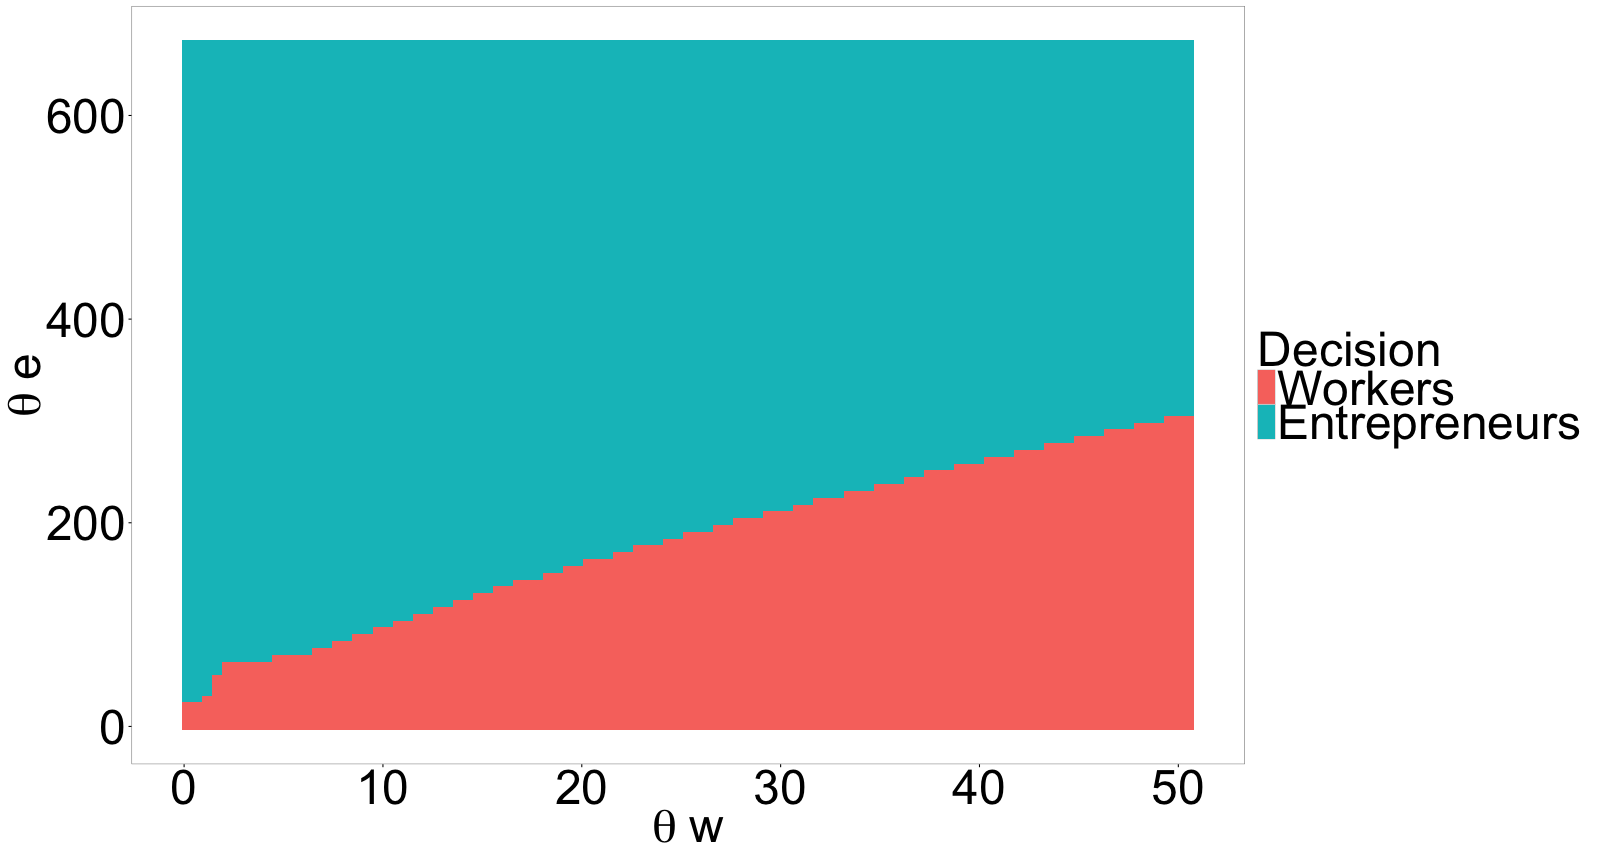
\includegraphics[width=1\textwidth]{/Users/rodrigoazuero/Dropbox/OptmalTaxationShared/Data/git/OptimalTaxation/TheoreticalMoments/EntreprenDecision.png}

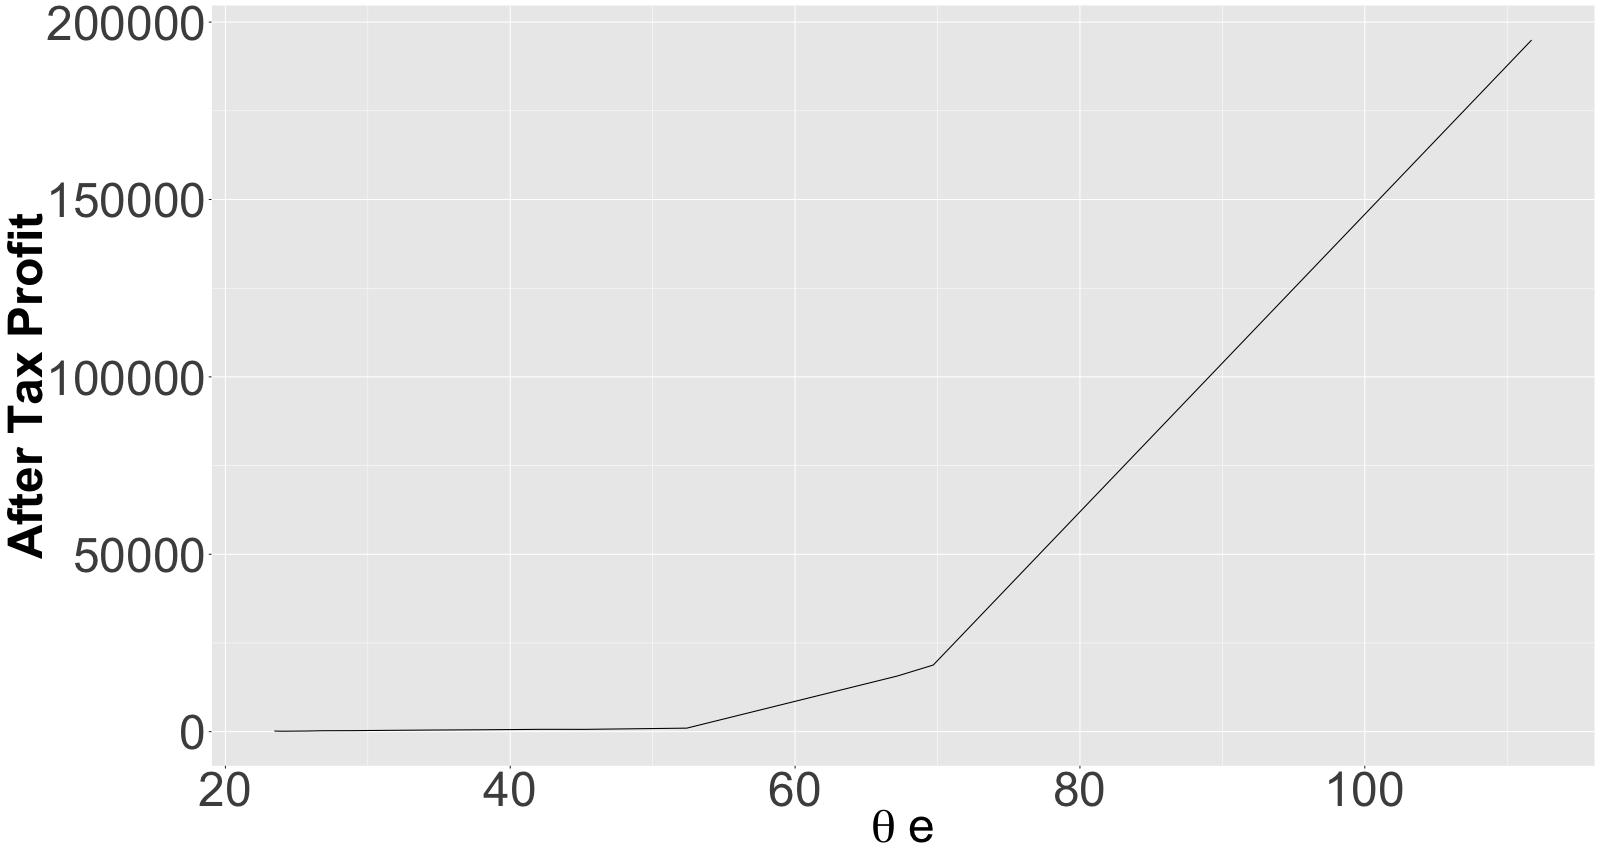
\includegraphics[width=1\textwidth]{/Users/rodrigoazuero/Dropbox/OptmalTaxationShared/Data/git/OptimalTaxation/TheoreticalMoments/AfterTaxProfit.png}

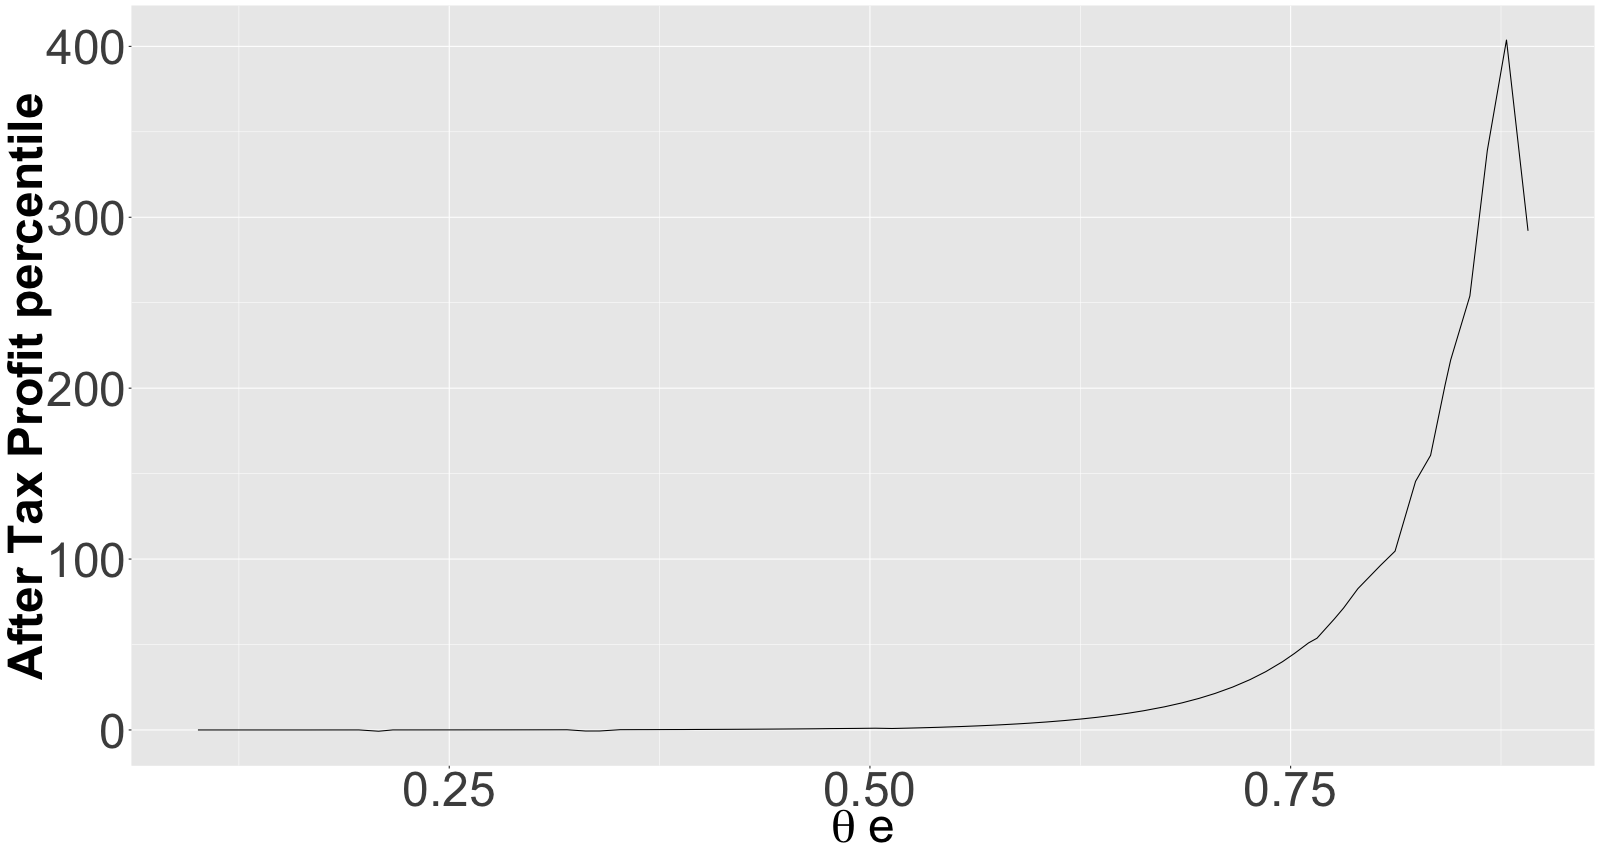
\includegraphics[width=1\textwidth]{/Users/rodrigoazuero/Dropbox/OptmalTaxationShared/Data/git/OptimalTaxation/TheoreticalMoments/AfterTaxProfitPercentile.png}


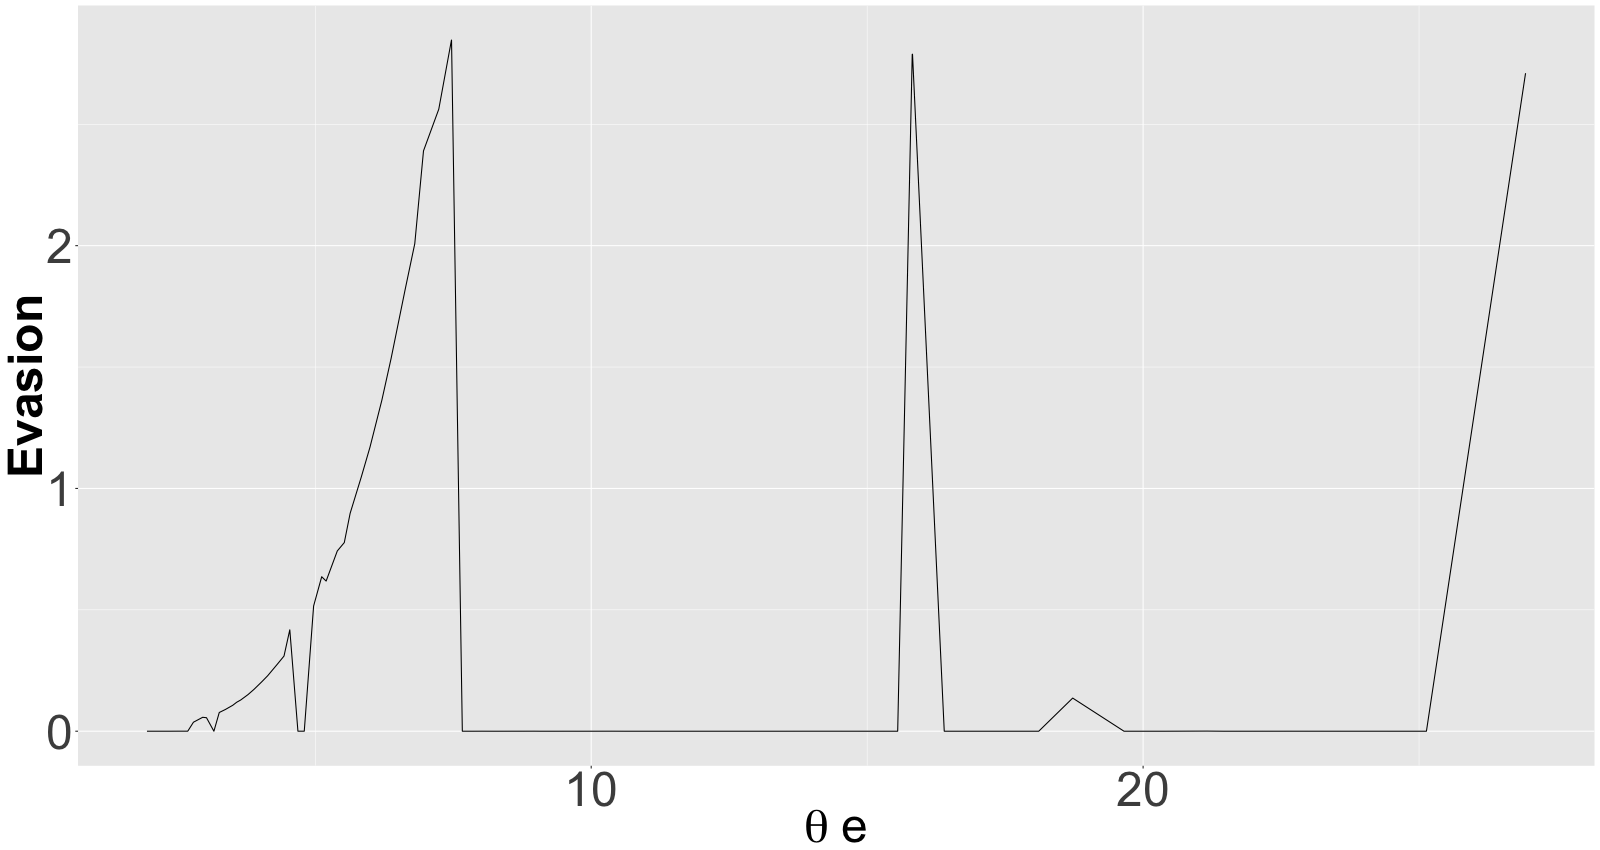
\includegraphics[width=1\textwidth]{/Users/rodrigoazuero/Dropbox/OptmalTaxationShared/Data/git/OptimalTaxation/TheoreticalMoments/EvasionProportion.png}

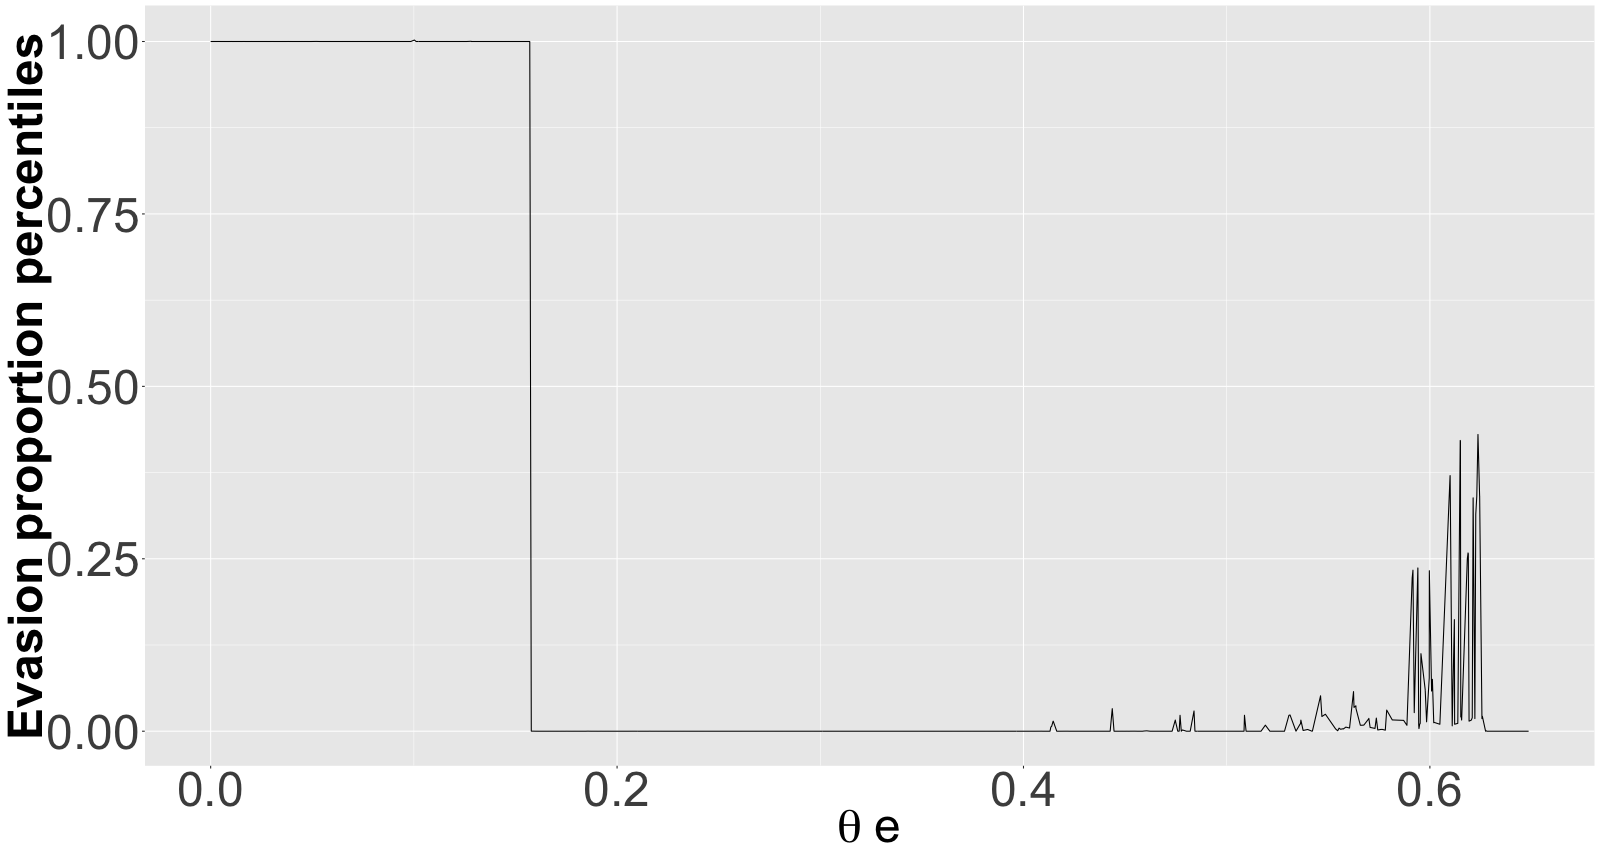
\includegraphics[width=1\textwidth]{/Users/rodrigoazuero/Dropbox/OptmalTaxationShared/Data/git/OptimalTaxation/TheoreticalMoments/EvasionProportionPercentiles.png}

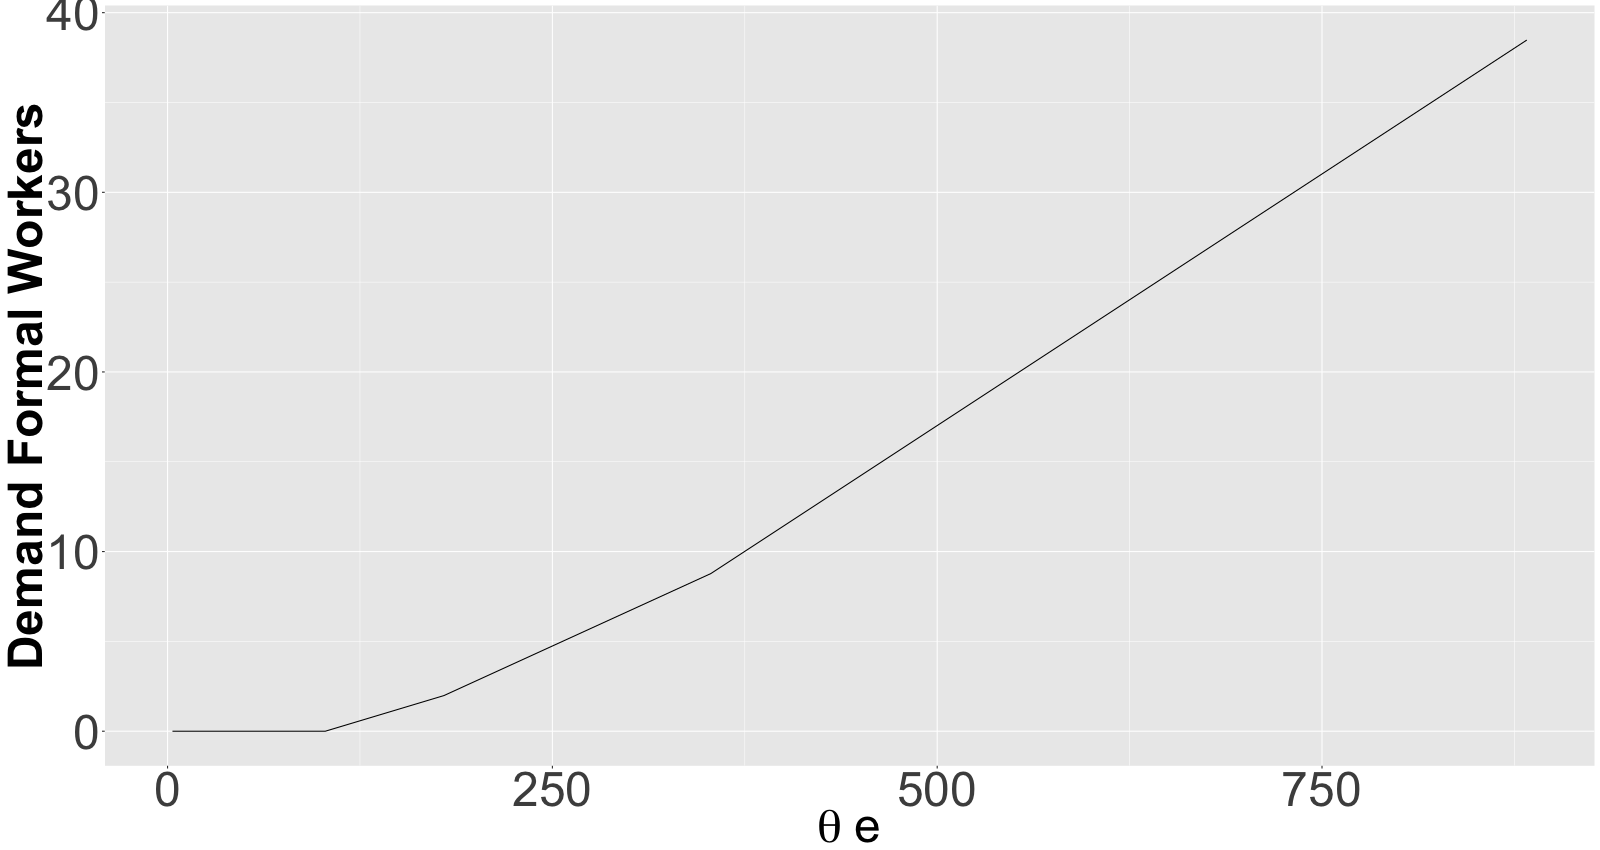
\includegraphics[width=1\textwidth]{/Users/rodrigoazuero/Dropbox/OptmalTaxationShared/Data/git/OptimalTaxation/TheoreticalMoments/FormalDemand.png}

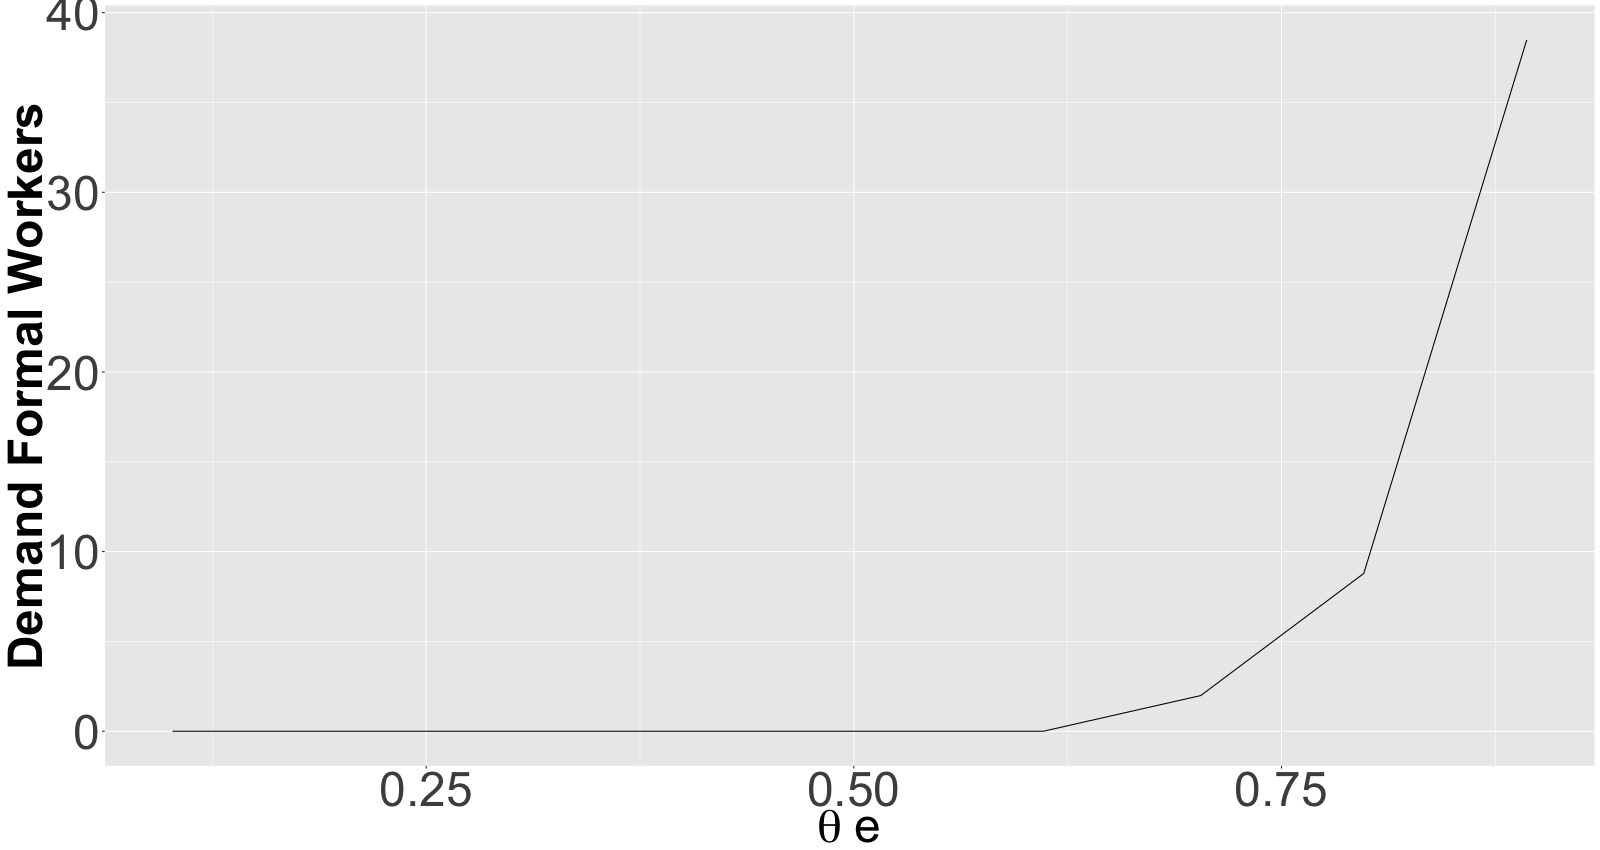
\includegraphics[width=1\textwidth]{/Users/rodrigoazuero/Dropbox/OptmalTaxationShared/Data/git/OptimalTaxation/TheoreticalMoments/FormalDemandPercentile.png}

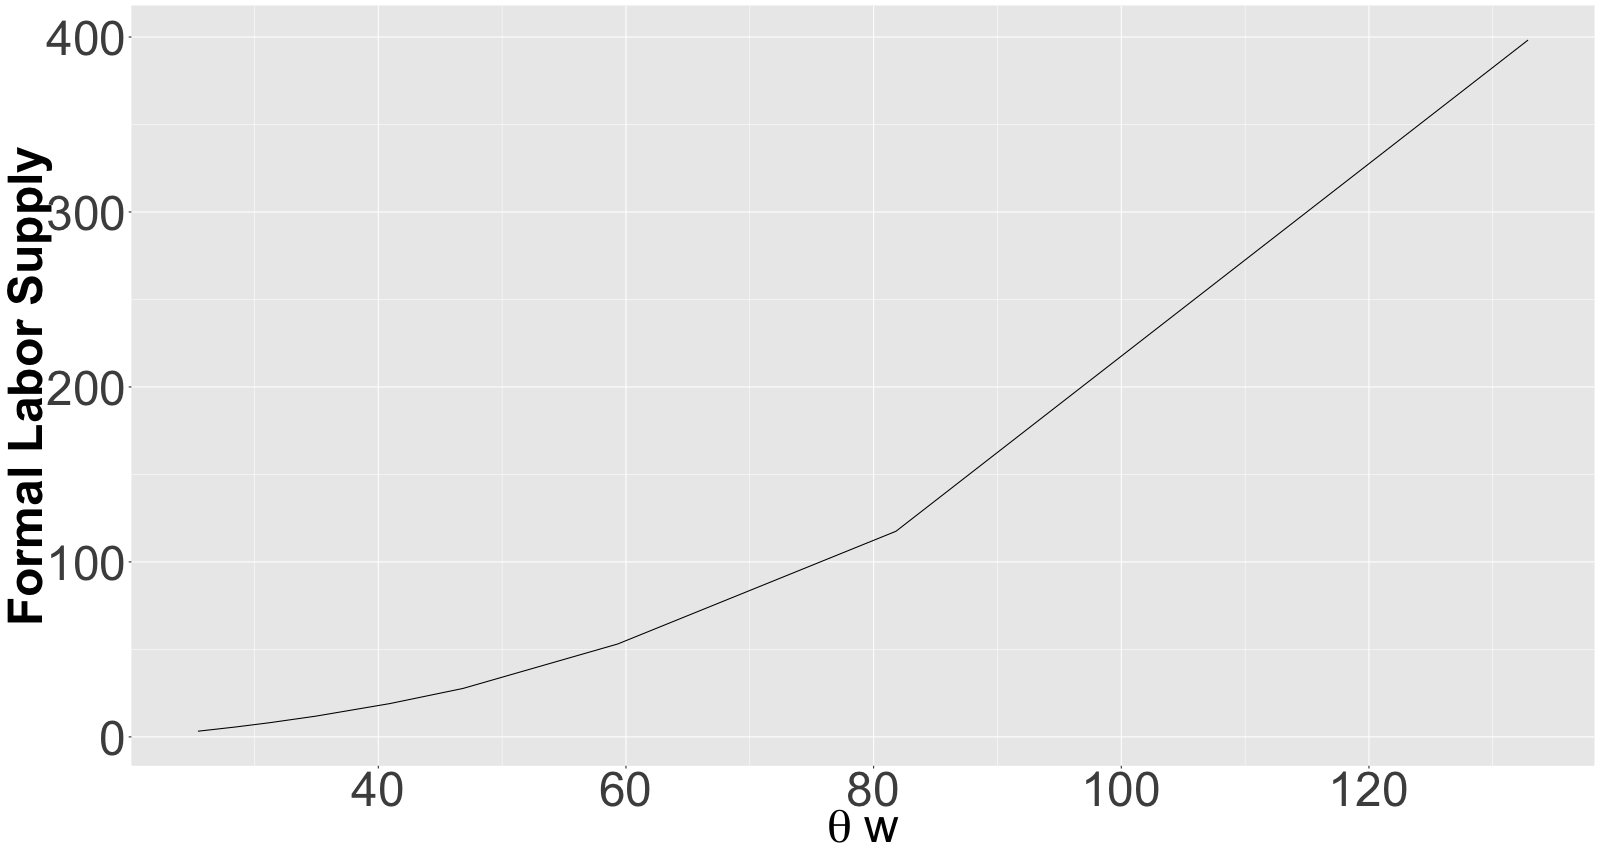
\includegraphics[width=1\textwidth]{/Users/rodrigoazuero/Dropbox/OptmalTaxationShared/Data/git/OptimalTaxation/TheoreticalMoments/FormalSupply.png}

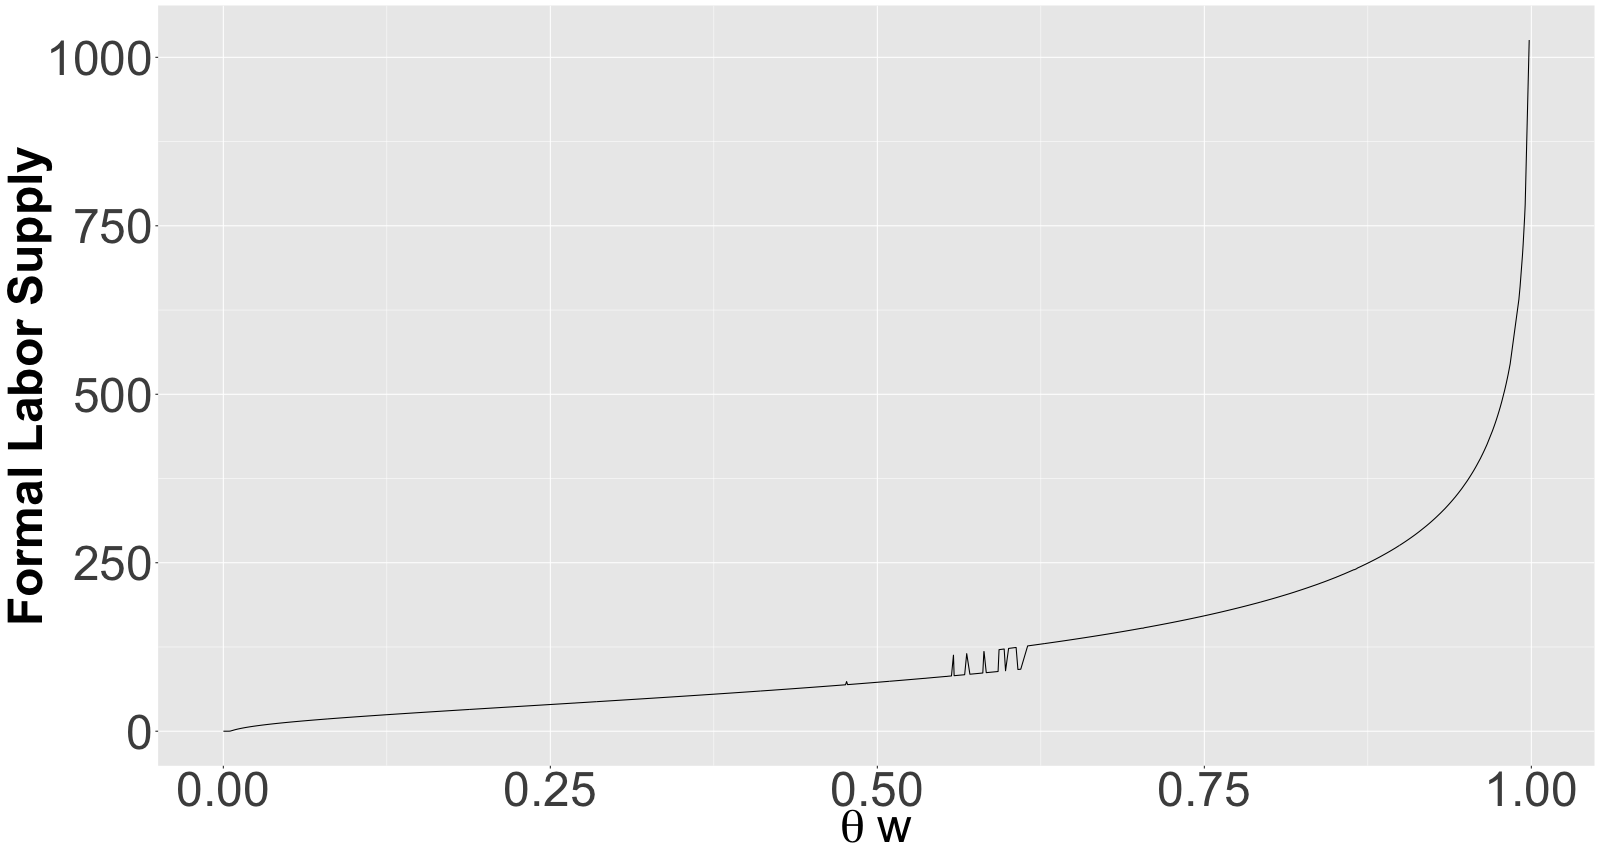
\includegraphics[width=1\textwidth]{/Users/rodrigoazuero/Dropbox/OptmalTaxationShared/Data/git/OptimalTaxation/TheoreticalMoments/FormalSupplyPercentiles.png}

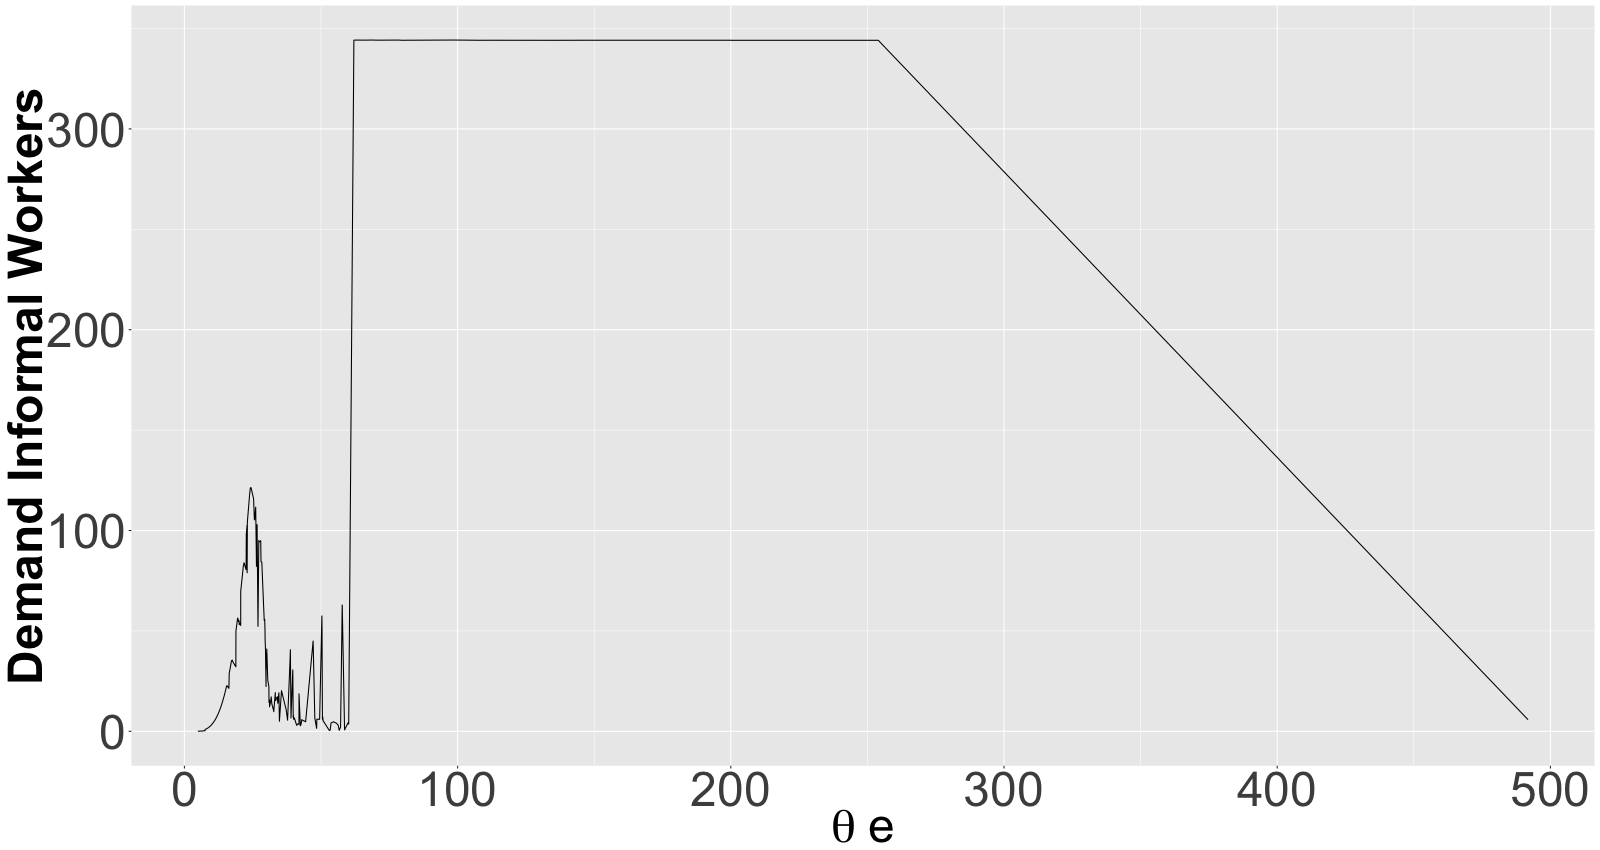
\includegraphics[width=1\textwidth]{/Users/rodrigoazuero/Dropbox/OptmalTaxationShared/Data/git/OptimalTaxation/TheoreticalMoments/InformalDemand.png}

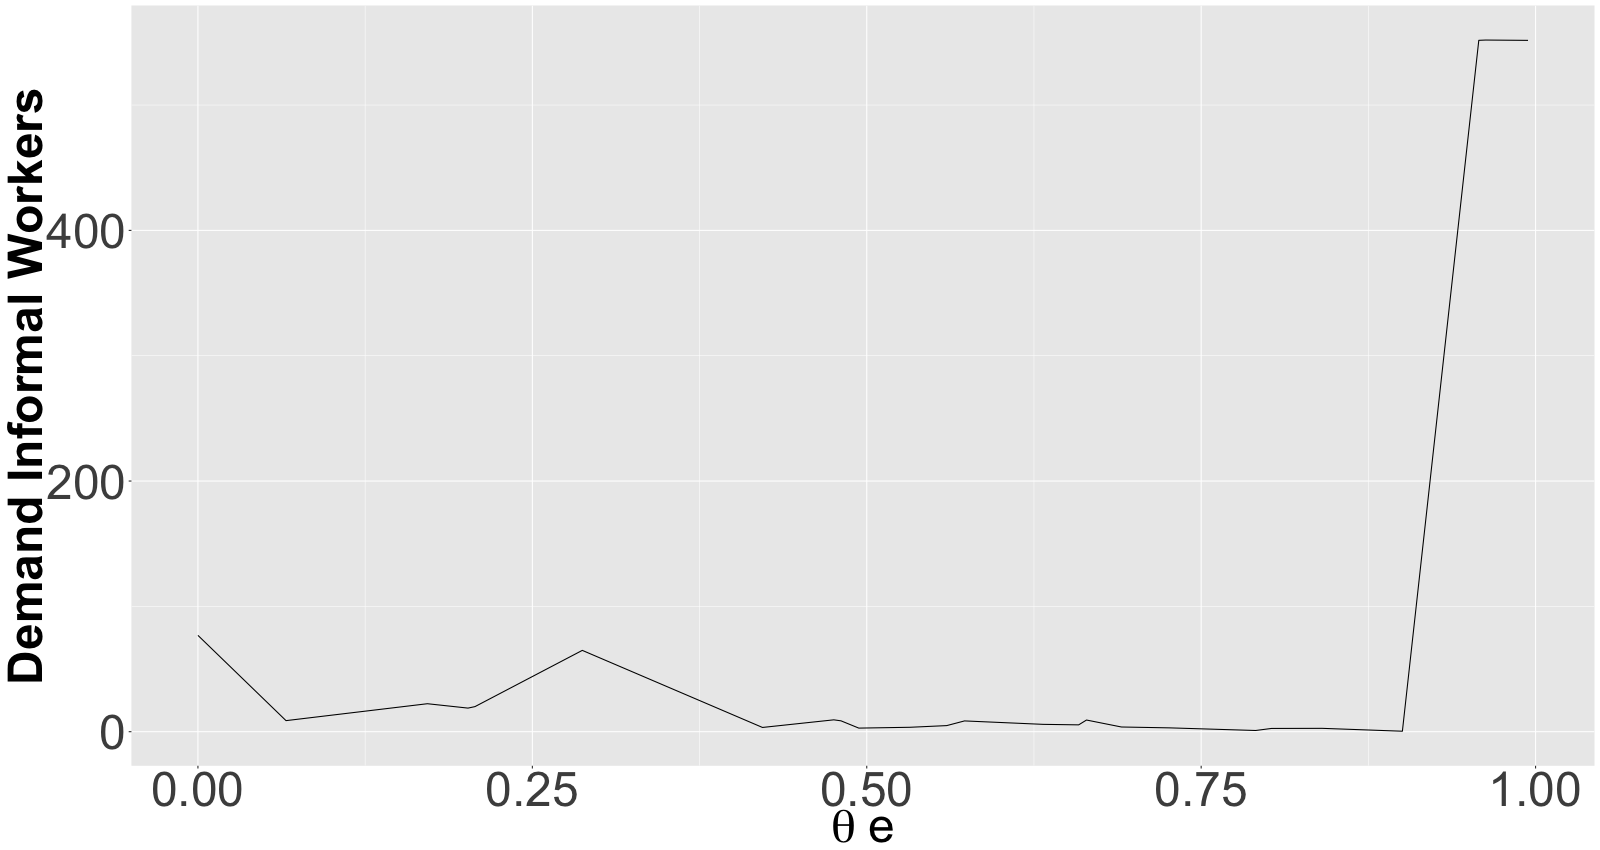
\includegraphics[width=1\textwidth]{/Users/rodrigoazuero/Dropbox/OptmalTaxationShared/Data/git/OptimalTaxation/TheoreticalMoments/InformalDemandPercentile.png}

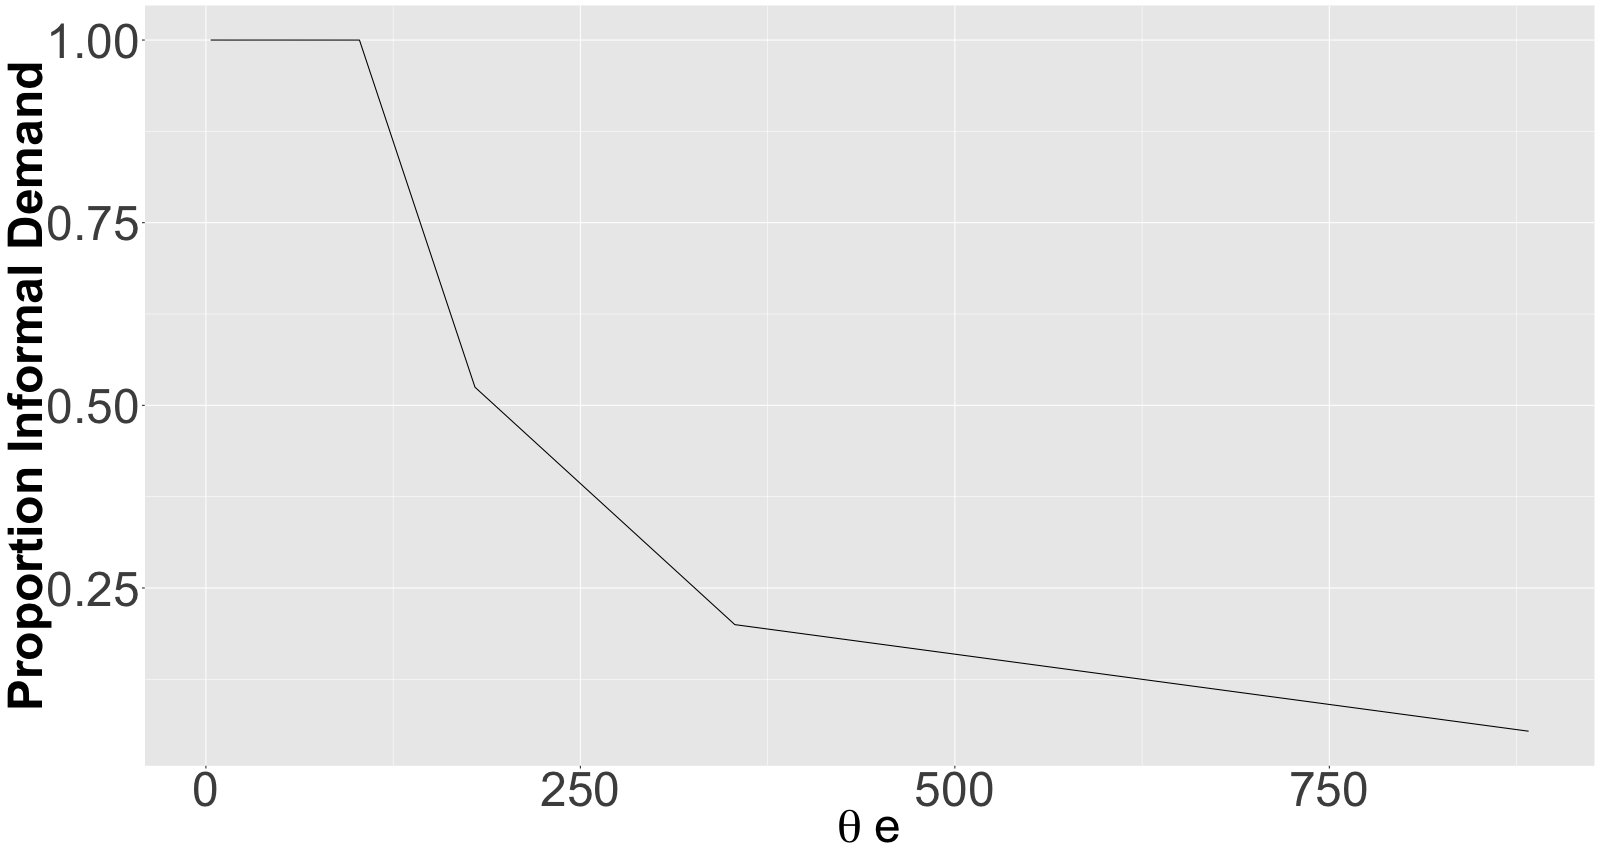
\includegraphics[width=1\textwidth]{/Users/rodrigoazuero/Dropbox/OptmalTaxationShared/Data/git/OptimalTaxation/TheoreticalMoments/InformalProportionDemand.png}

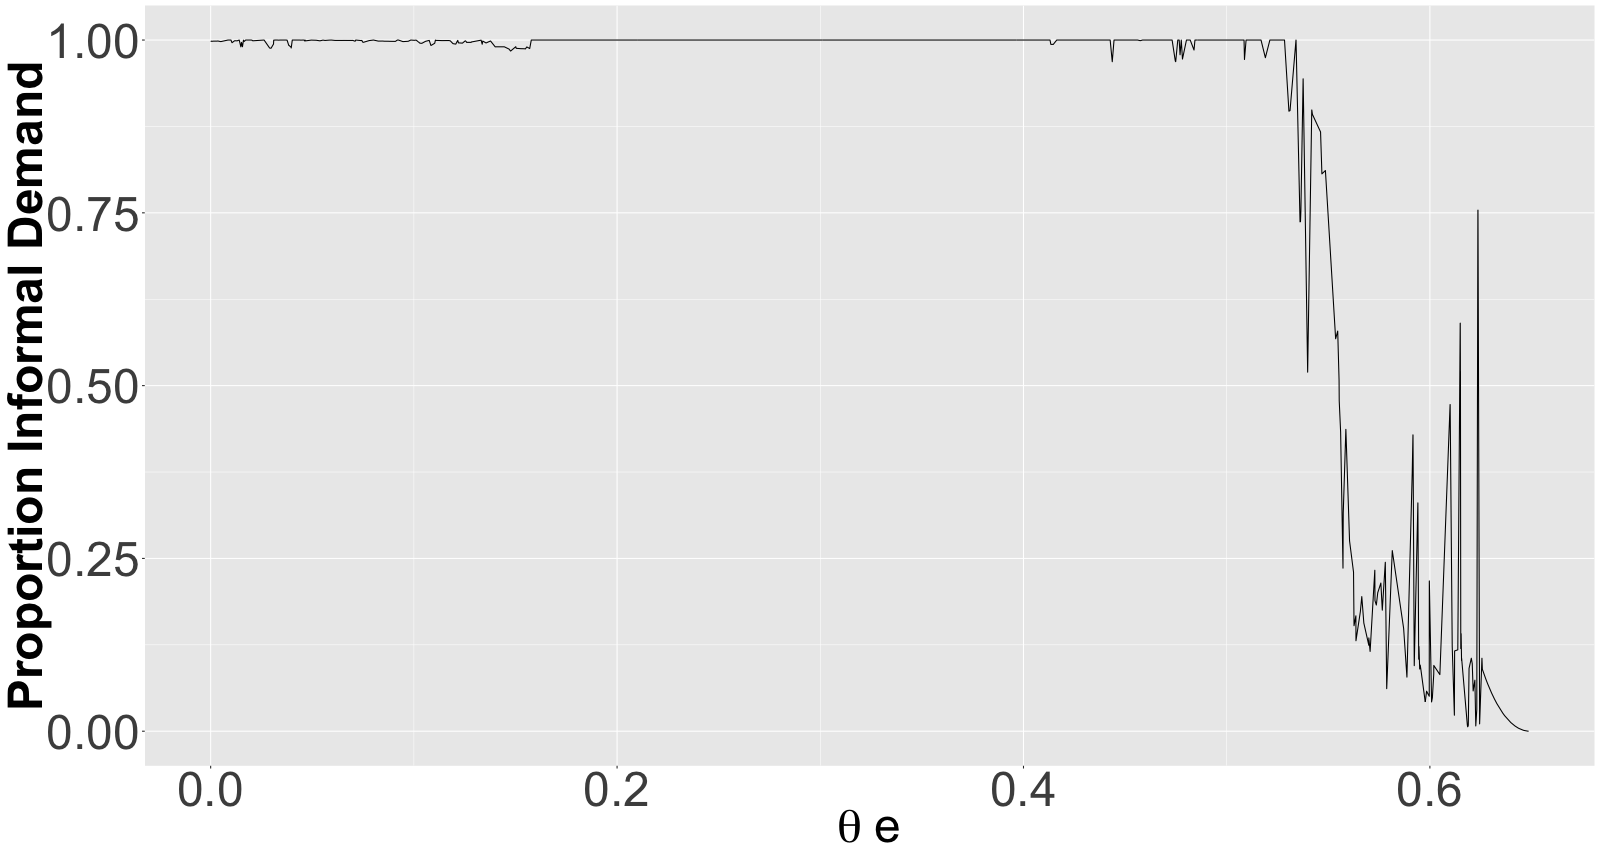
\includegraphics[width=1\textwidth]{/Users/rodrigoazuero/Dropbox/OptmalTaxationShared/Data/git/OptimalTaxation/TheoreticalMoments/InformalProportionDemandPercentile.png}

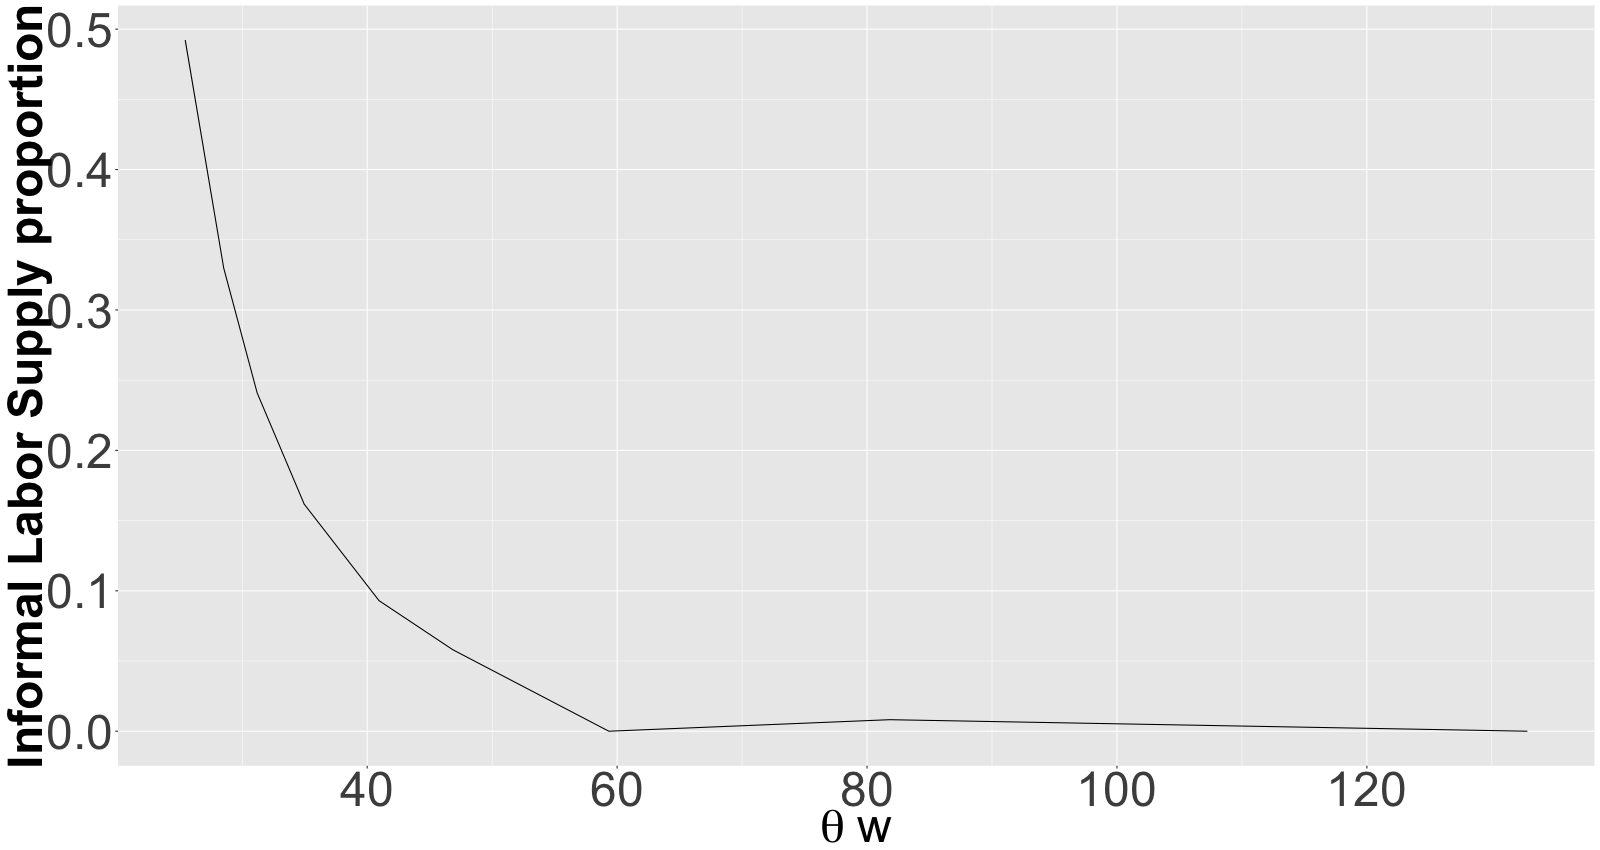
\includegraphics[width=1\textwidth]{/Users/rodrigoazuero/Dropbox/OptmalTaxationShared/Data/git/OptimalTaxation/TheoreticalMoments/InformalProportionSupply.png}

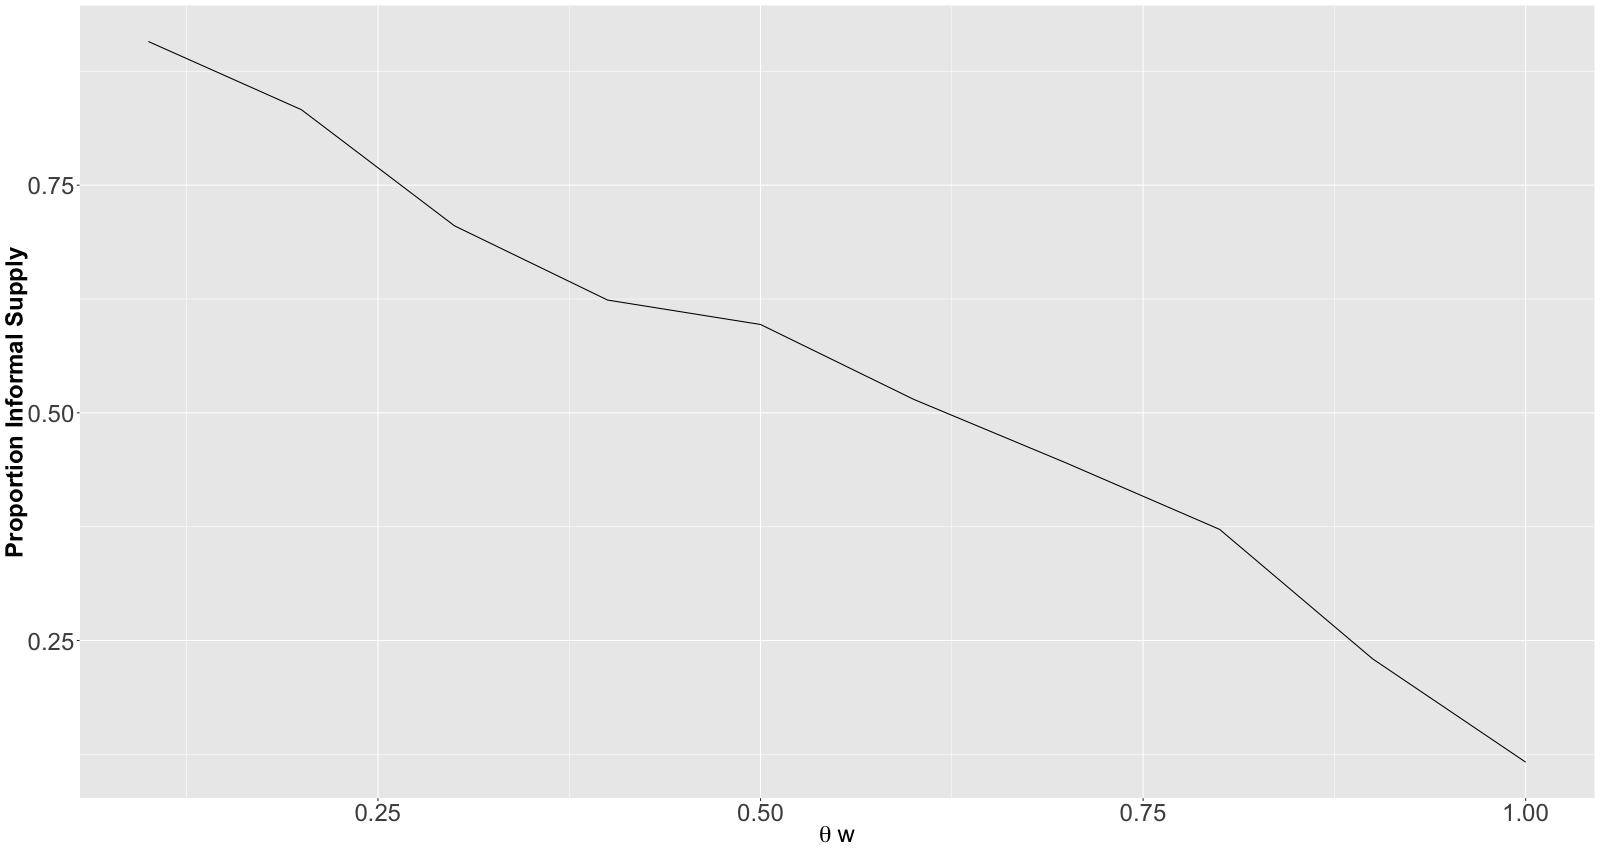
\includegraphics[width=1\textwidth]{/Users/rodrigoazuero/Dropbox/OptmalTaxationShared/Data/git/OptimalTaxation/TheoreticalMoments/InformalProportionSupplyPercentiles.png}

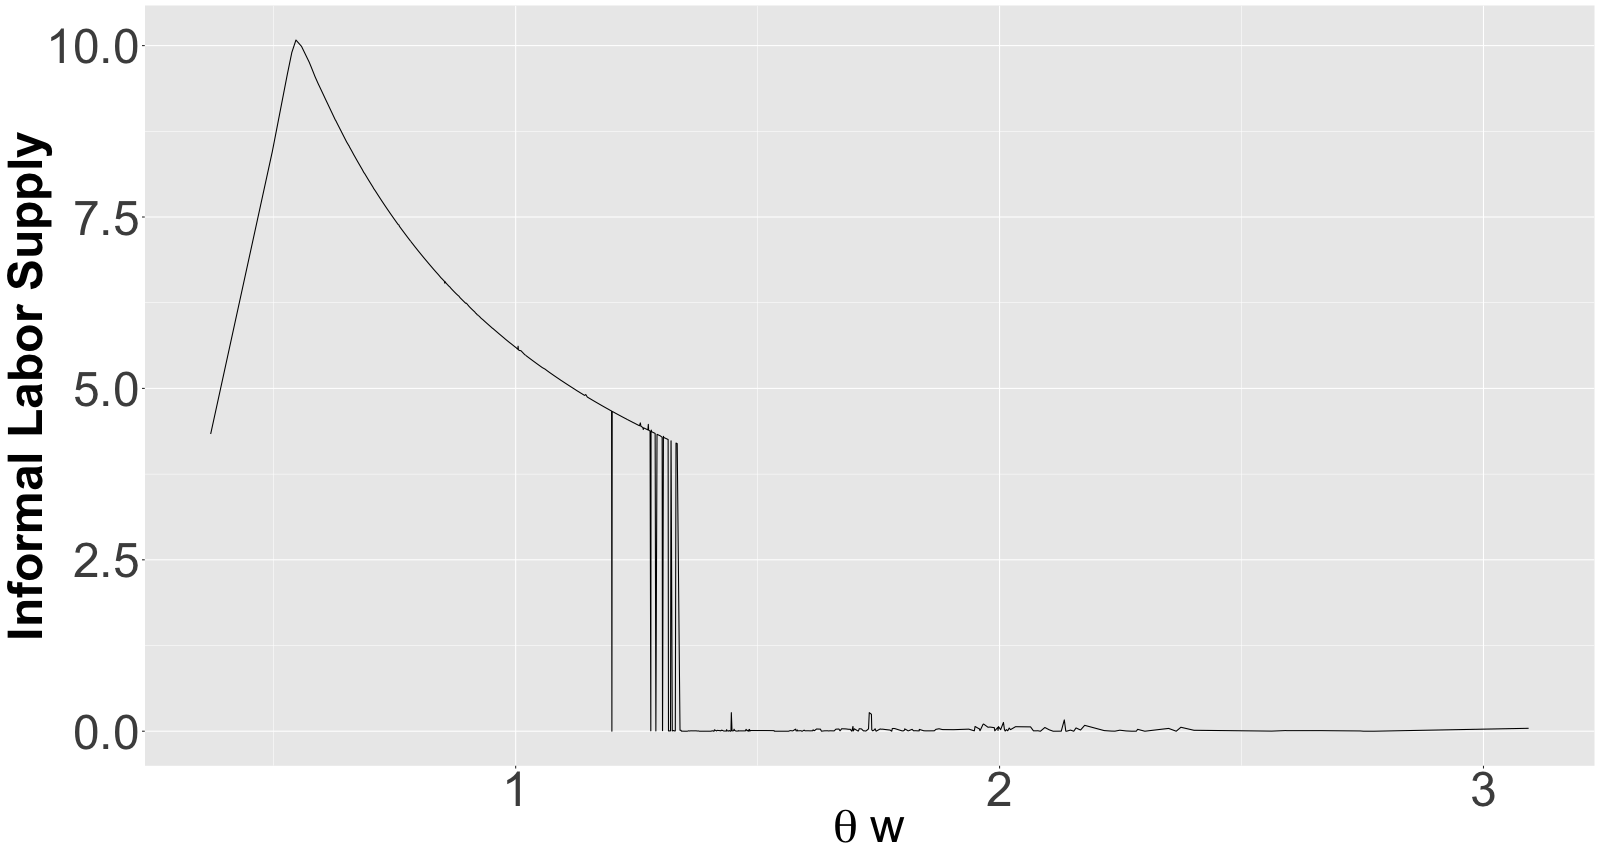
\includegraphics[width=1\textwidth]{/Users/rodrigoazuero/Dropbox/OptmalTaxationShared/Data/git/OptimalTaxation/TheoreticalMoments/InformalSupply.png}

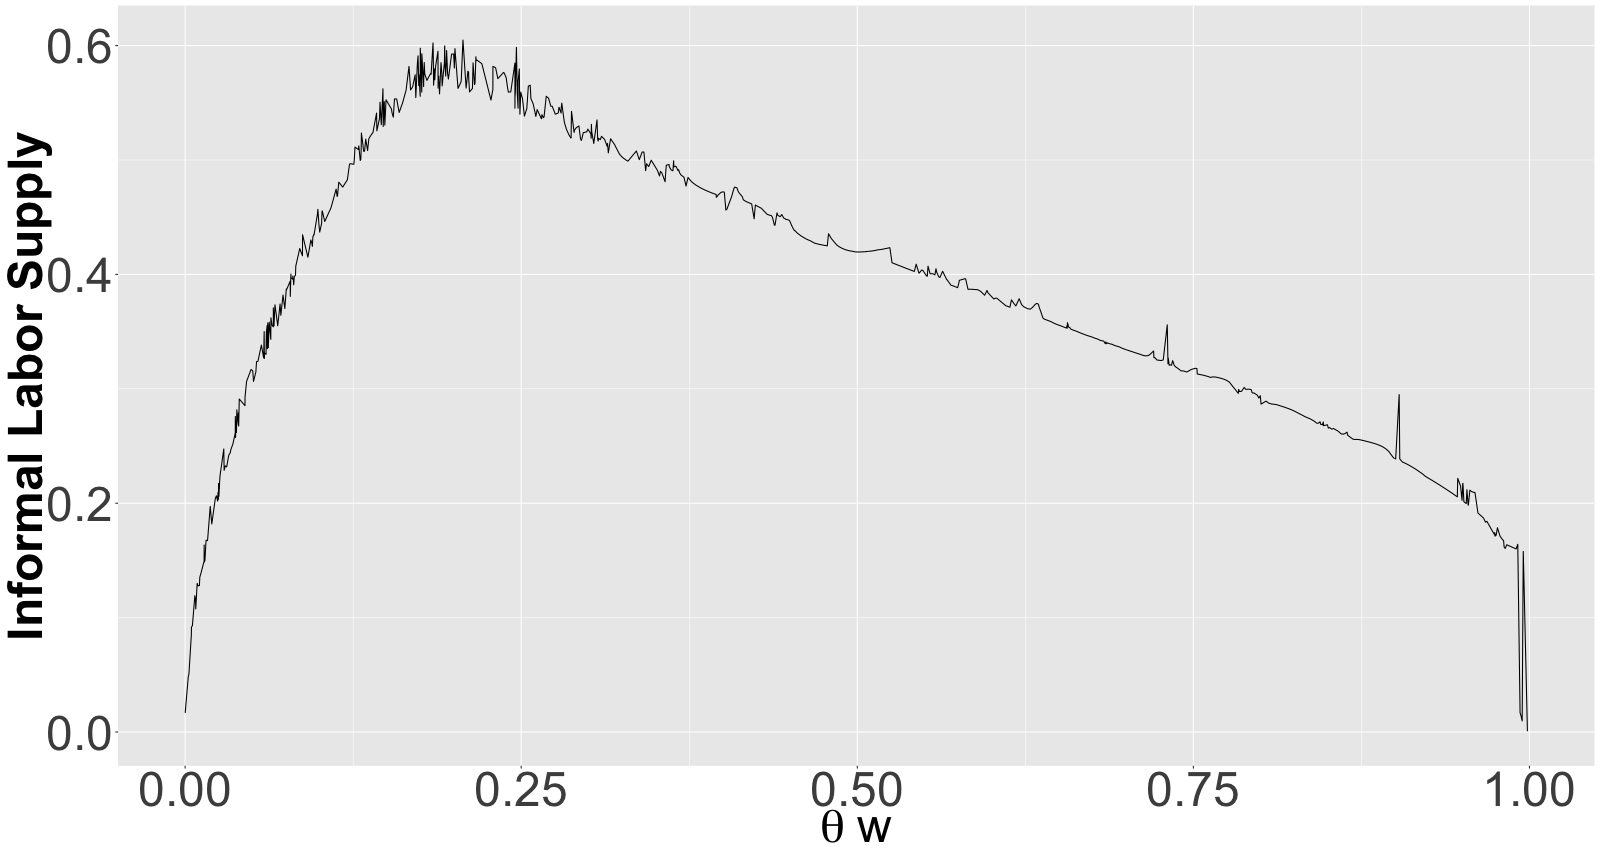
\includegraphics[width=1\textwidth]{/Users/rodrigoazuero/Dropbox/OptmalTaxationShared/Data/git/OptimalTaxation/TheoreticalMoments/InformalSupplyPercentiles.png}

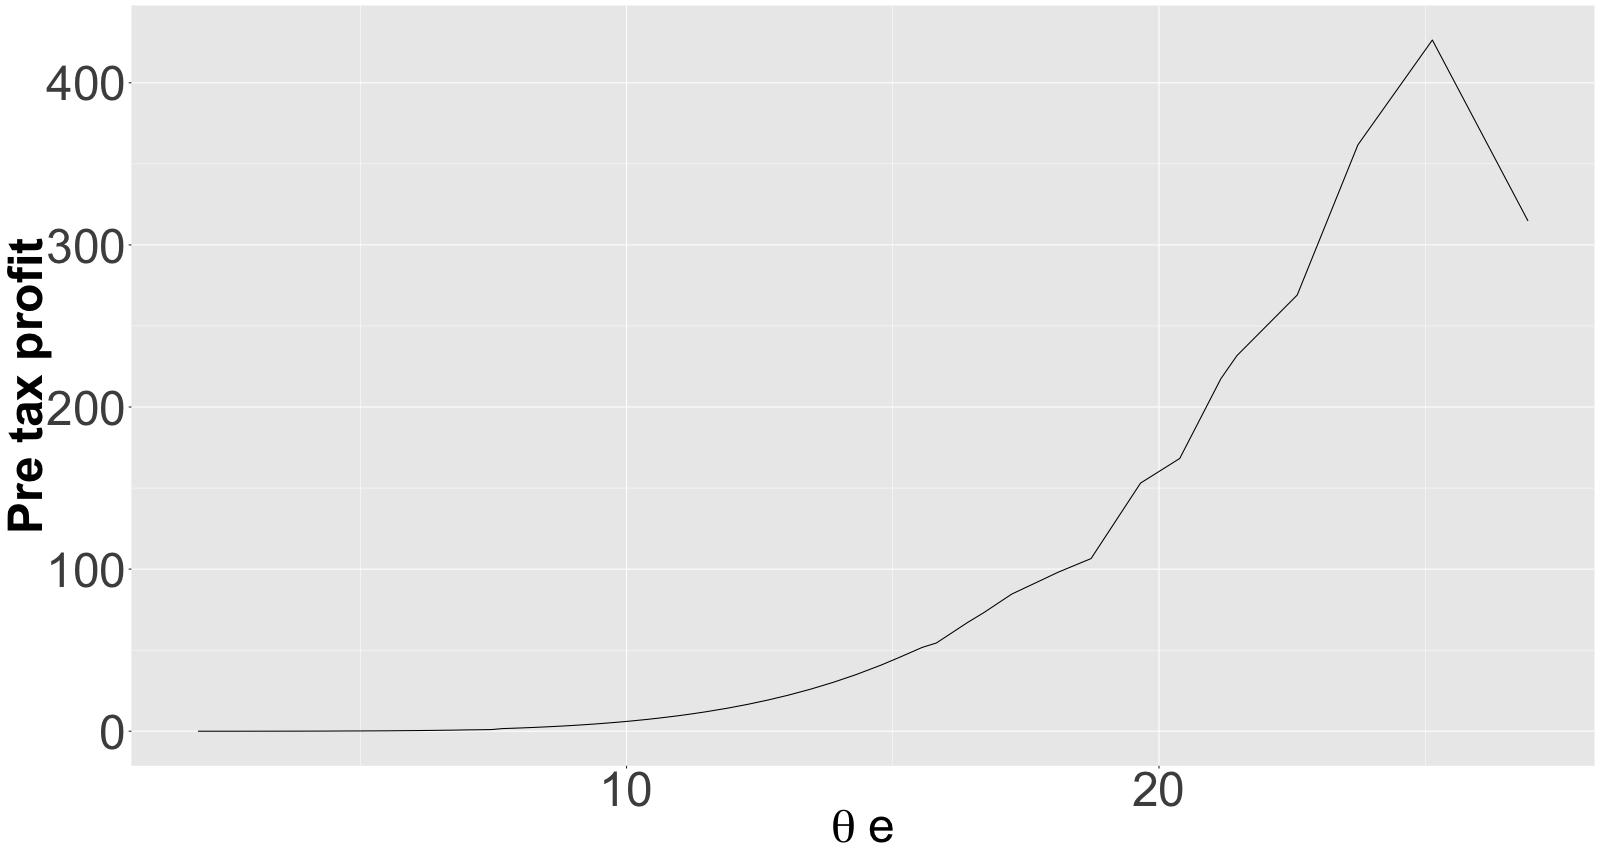
\includegraphics[width=1\textwidth]{/Users/rodrigoazuero/Dropbox/OptmalTaxationShared/Data/git/OptimalTaxation/TheoreticalMoments/PretaxProfit.png}

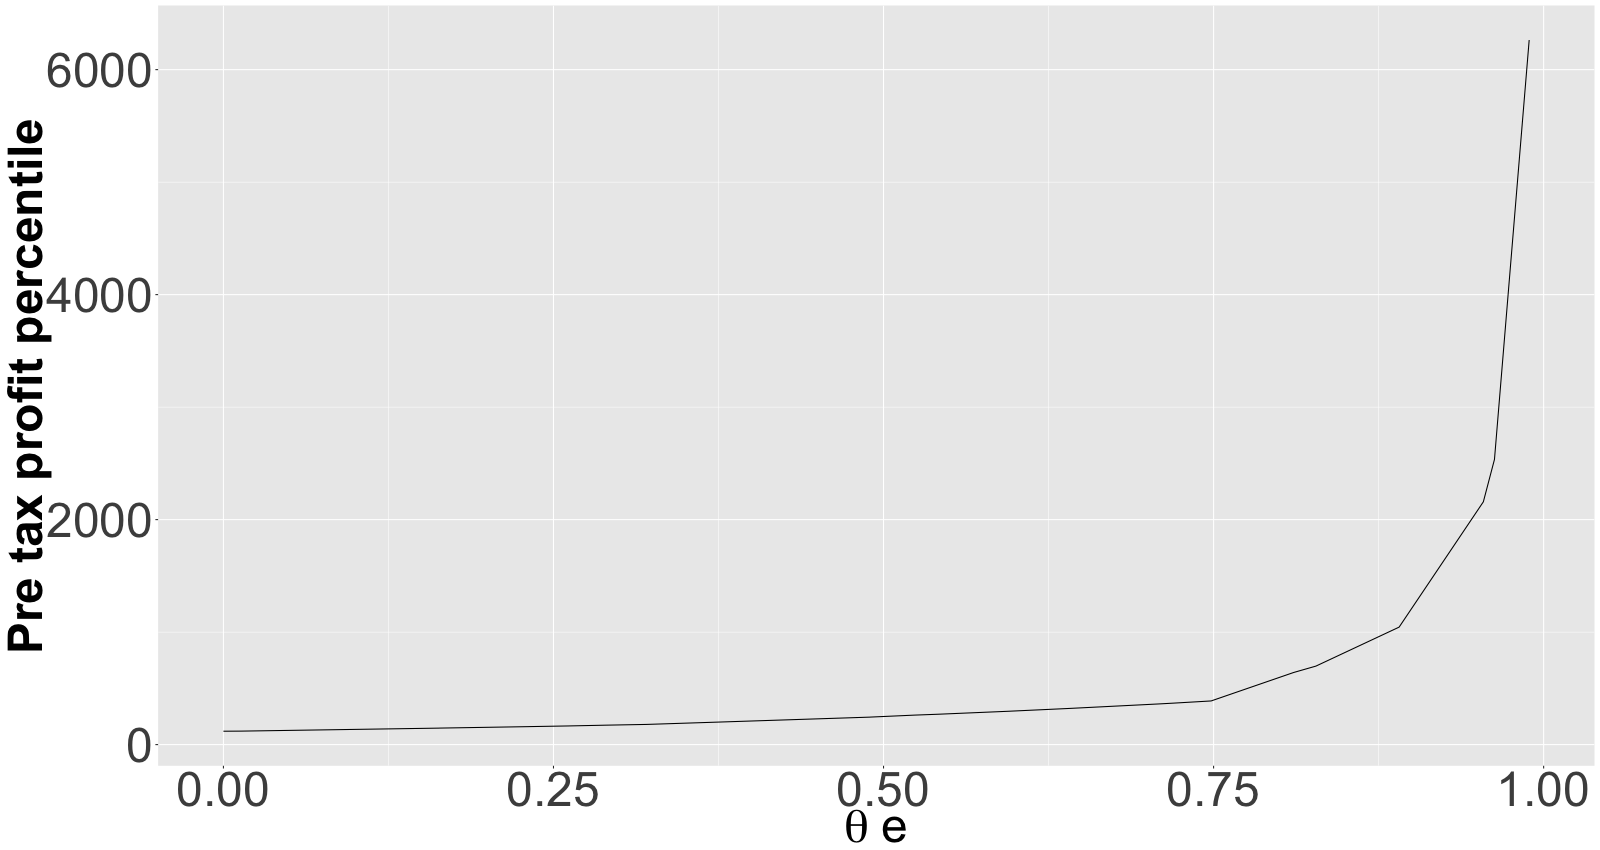
\includegraphics[width=1\textwidth]{/Users/rodrigoazuero/Dropbox/OptmalTaxationShared/Data/git/OptimalTaxation/TheoreticalMoments/PretaxProfitPercentile.png}

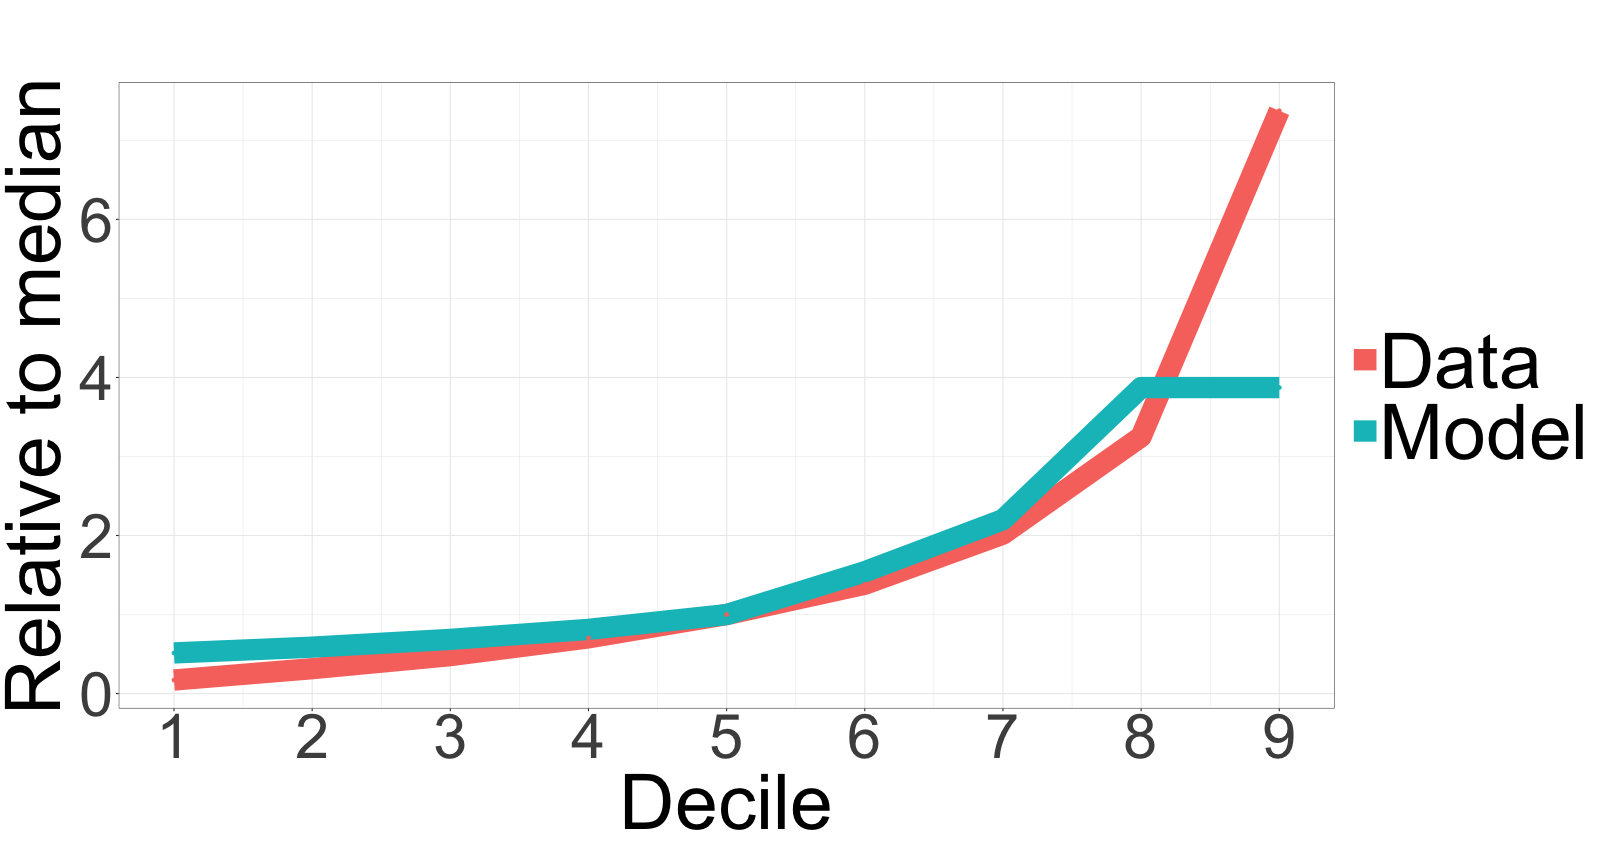
\includegraphics[width=1\textwidth]{/Users/rodrigoazuero/Dropbox/OptmalTaxationShared/Data/git/OptimalTaxation/TheoreticalMoments/Production.png}

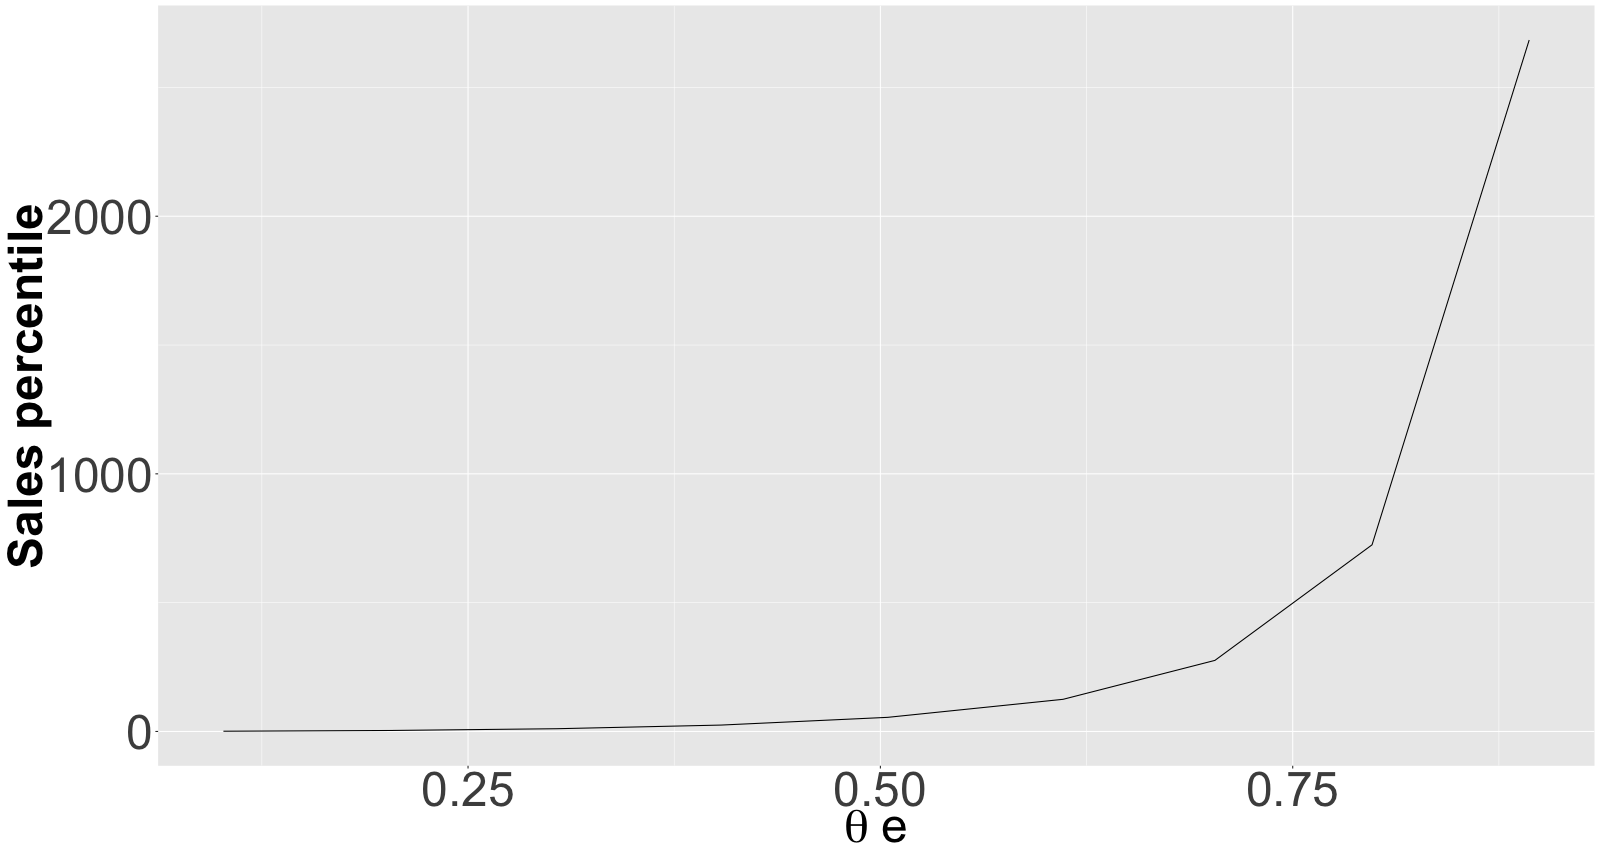
\includegraphics[width=1\textwidth]{/Users/rodrigoazuero/Dropbox/OptmalTaxationShared/Data/git/OptimalTaxation/TheoreticalMoments/ProductionPercentile.png}

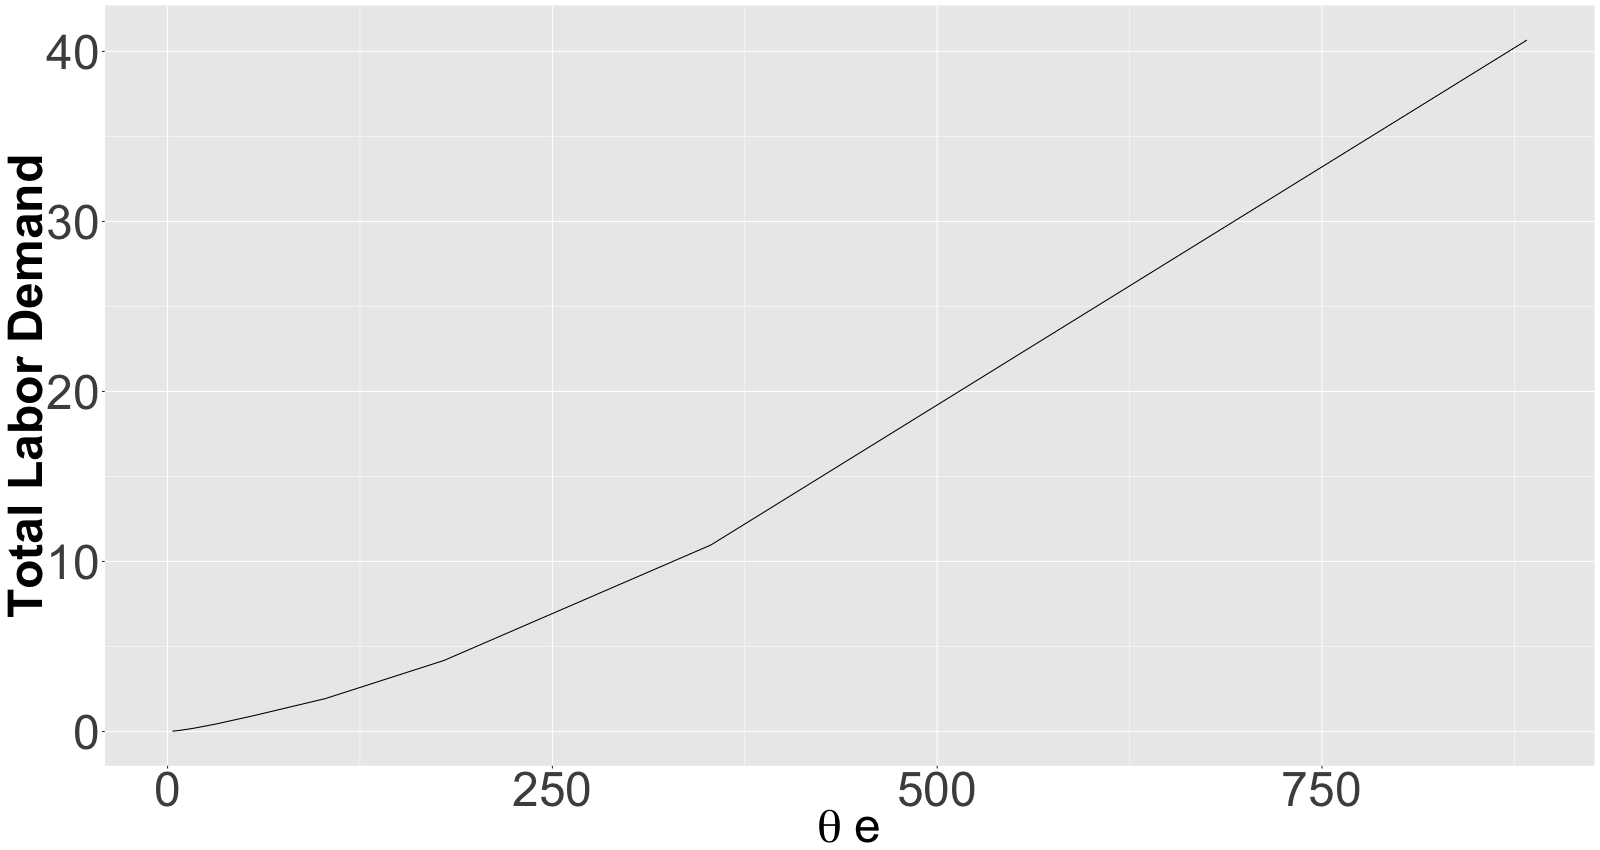
\includegraphics[width=1\textwidth]{/Users/rodrigoazuero/Dropbox/OptmalTaxationShared/Data/git/OptimalTaxation/TheoreticalMoments/TotalLaborDemand.png}

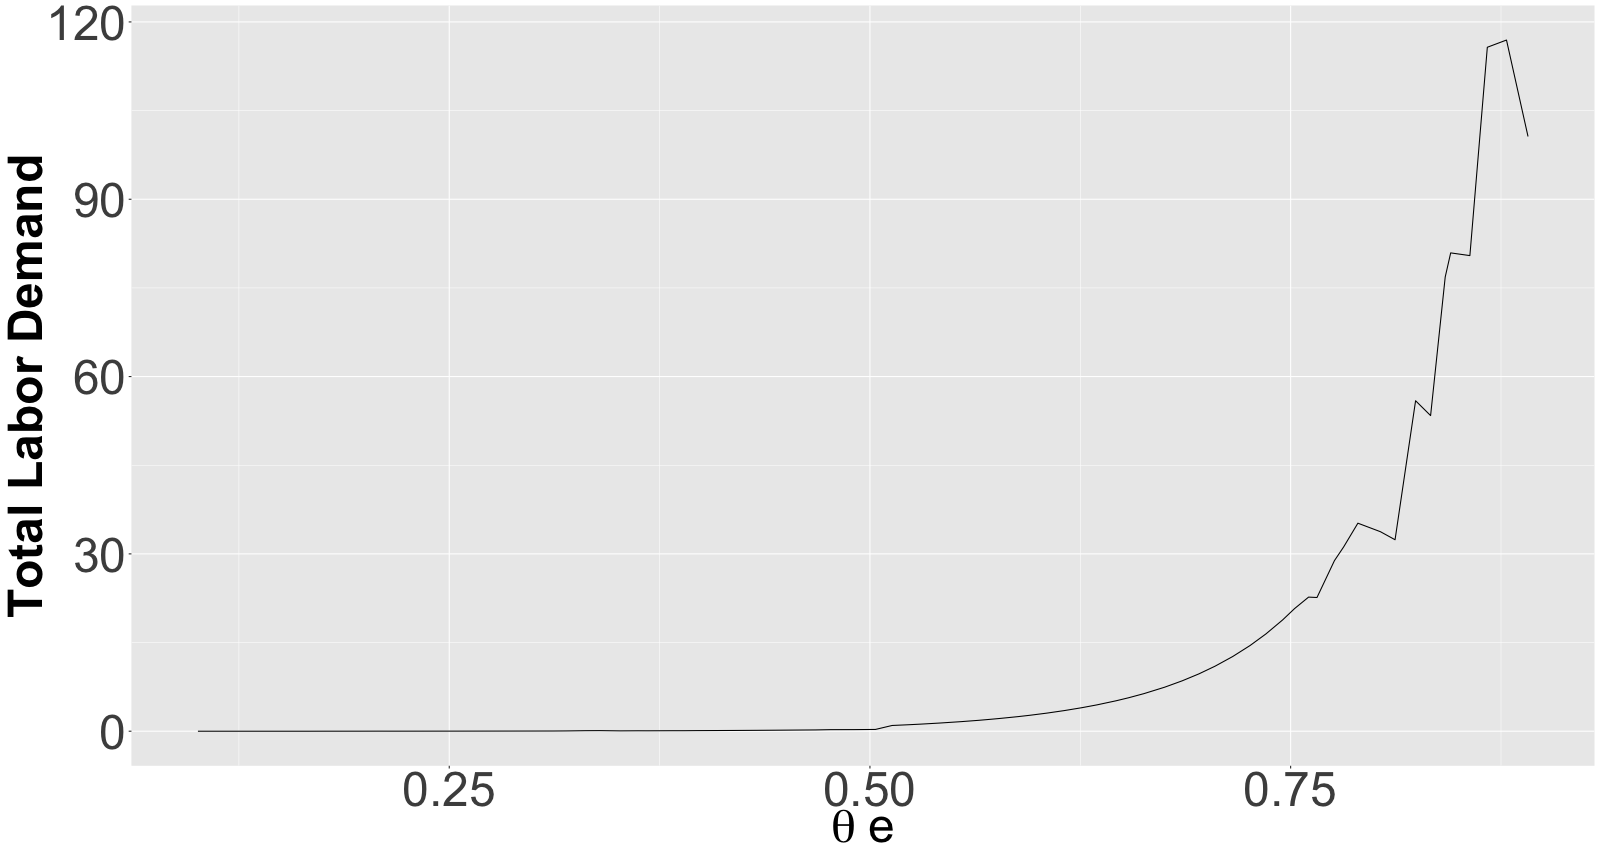
\includegraphics[width=1\textwidth]{/Users/rodrigoazuero/Dropbox/OptmalTaxationShared/Data/git/OptimalTaxation/TheoreticalMoments/TotalLaborDemandPercentile.png}

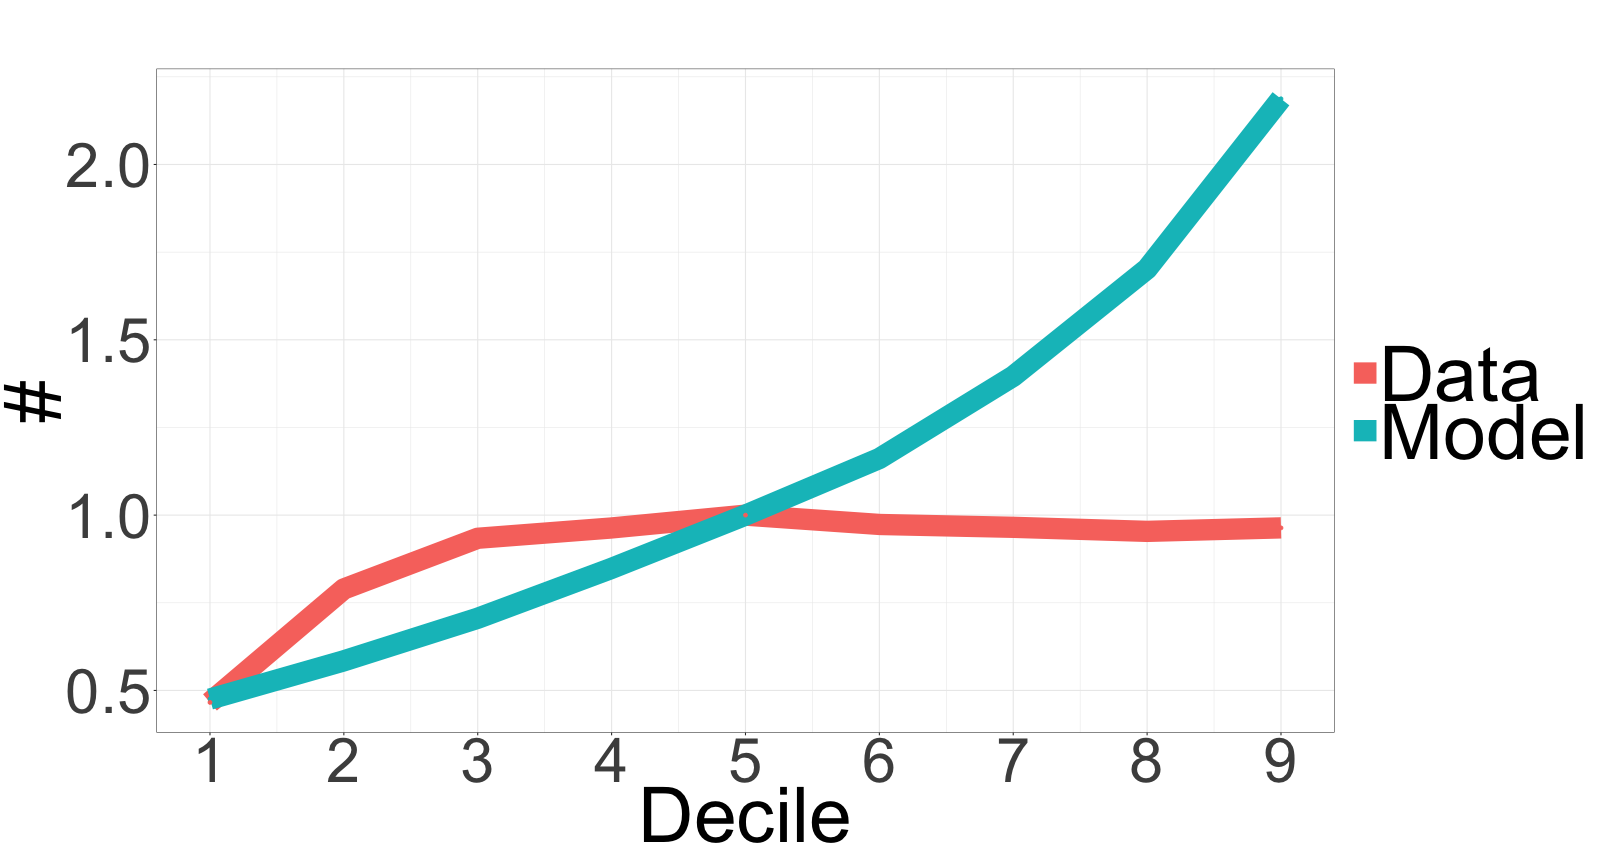
\includegraphics[width=1\textwidth]{/Users/rodrigoazuero/Dropbox/OptmalTaxationShared/Data/git/OptimalTaxation/TheoreticalMoments/TotalLaborSupply.png}

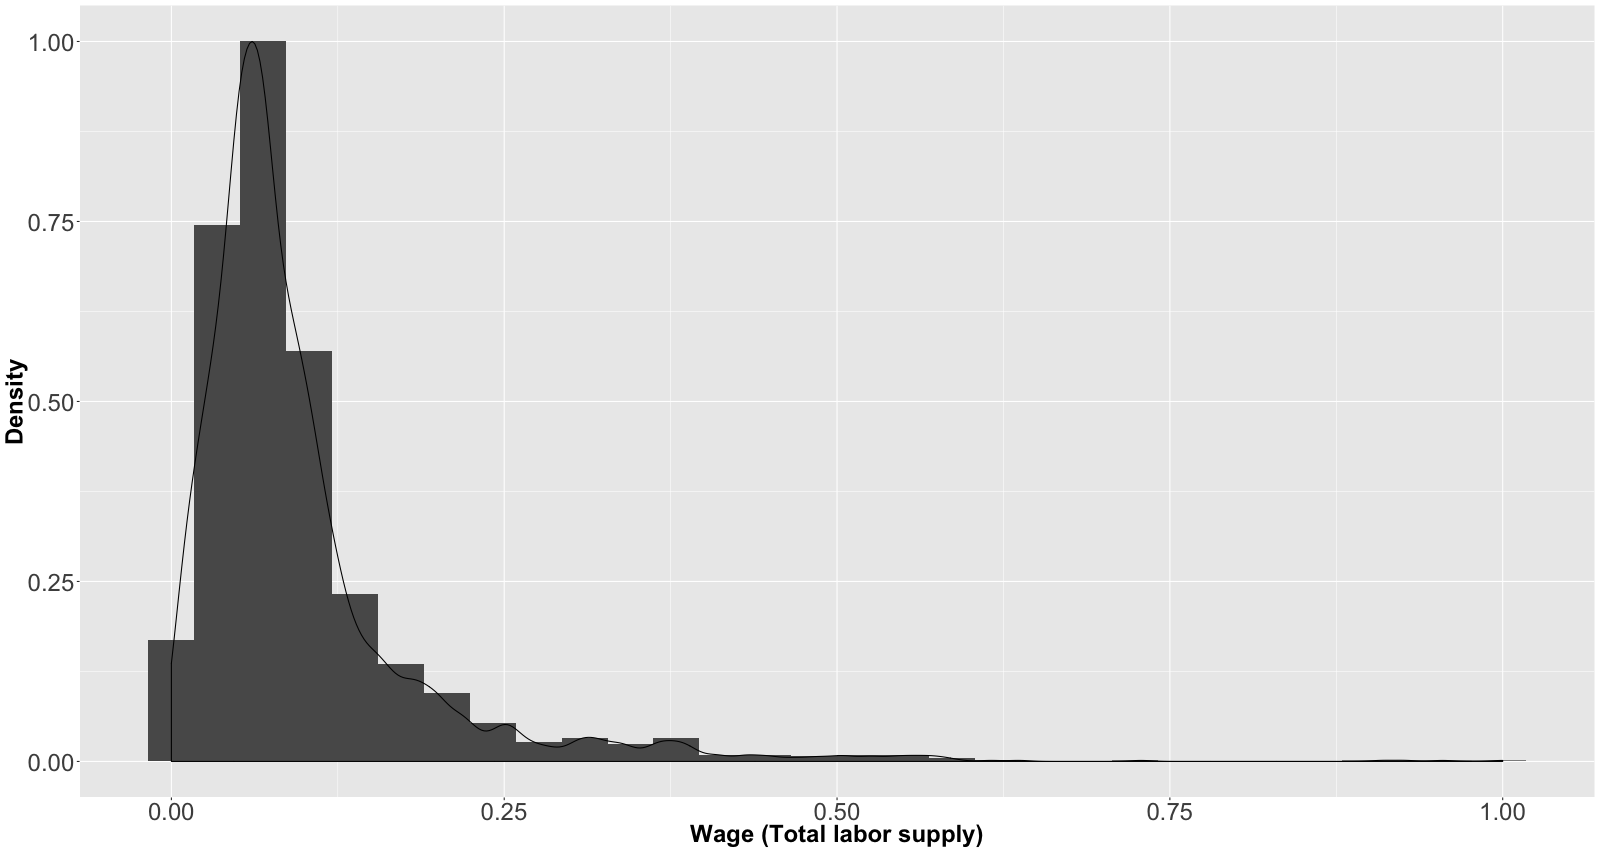
\includegraphics[width=1\textwidth]{/Users/rodrigoazuero/Dropbox/OptmalTaxationShared/Data/git/OptimalTaxation/TheoreticalMoments/TotalLaborSupplyPercentiles.png}

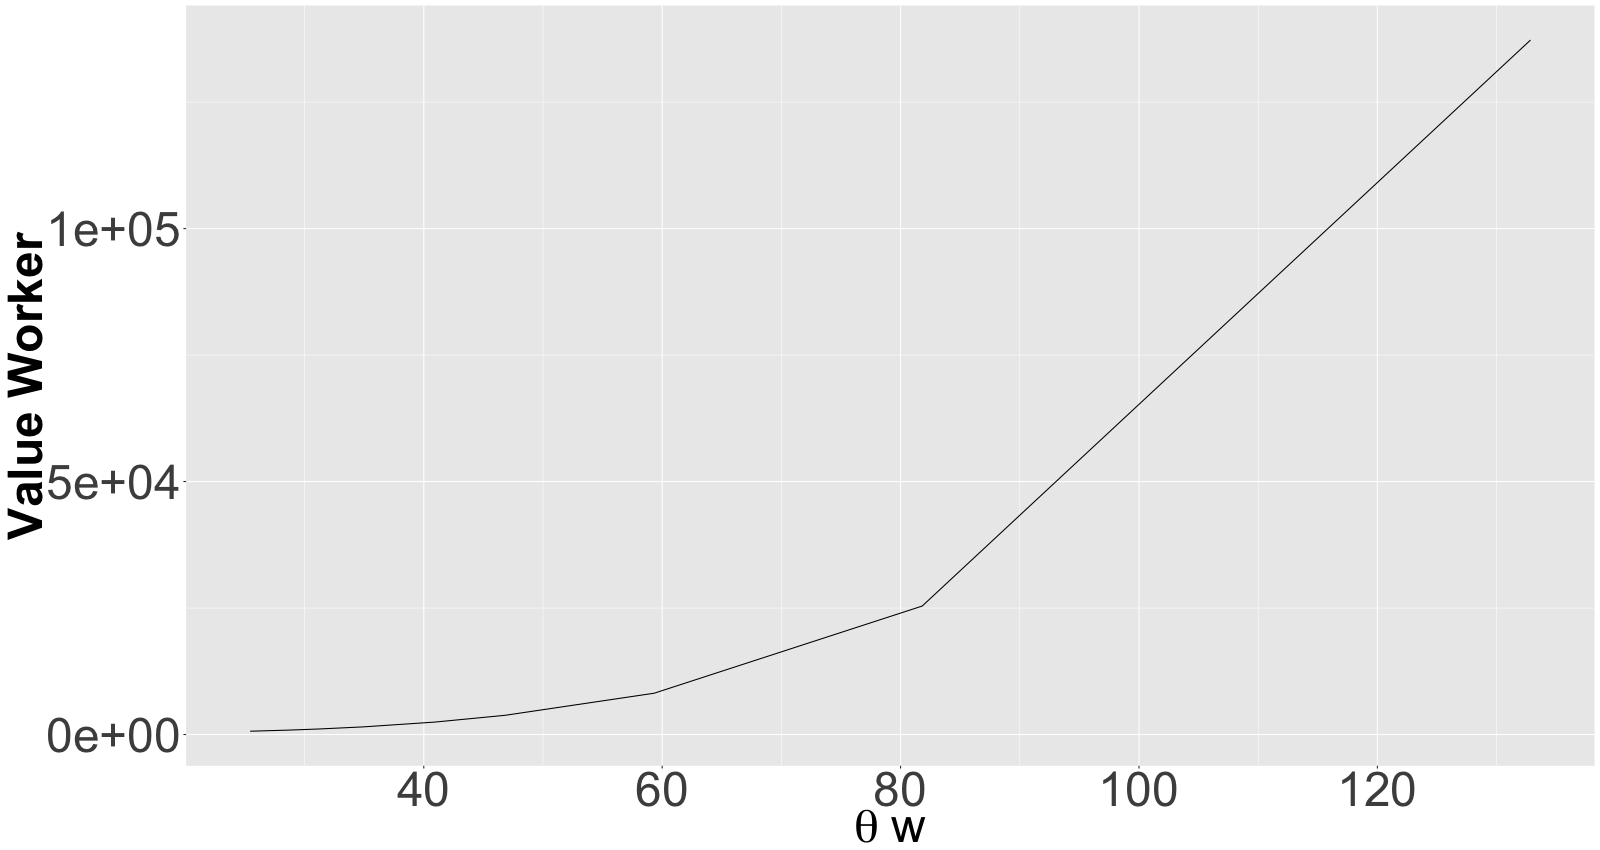
\includegraphics[width=1\textwidth]{/Users/rodrigoazuero/Dropbox/OptmalTaxationShared/Data/git/OptimalTaxation/TheoreticalMoments/ValueWorker.png}

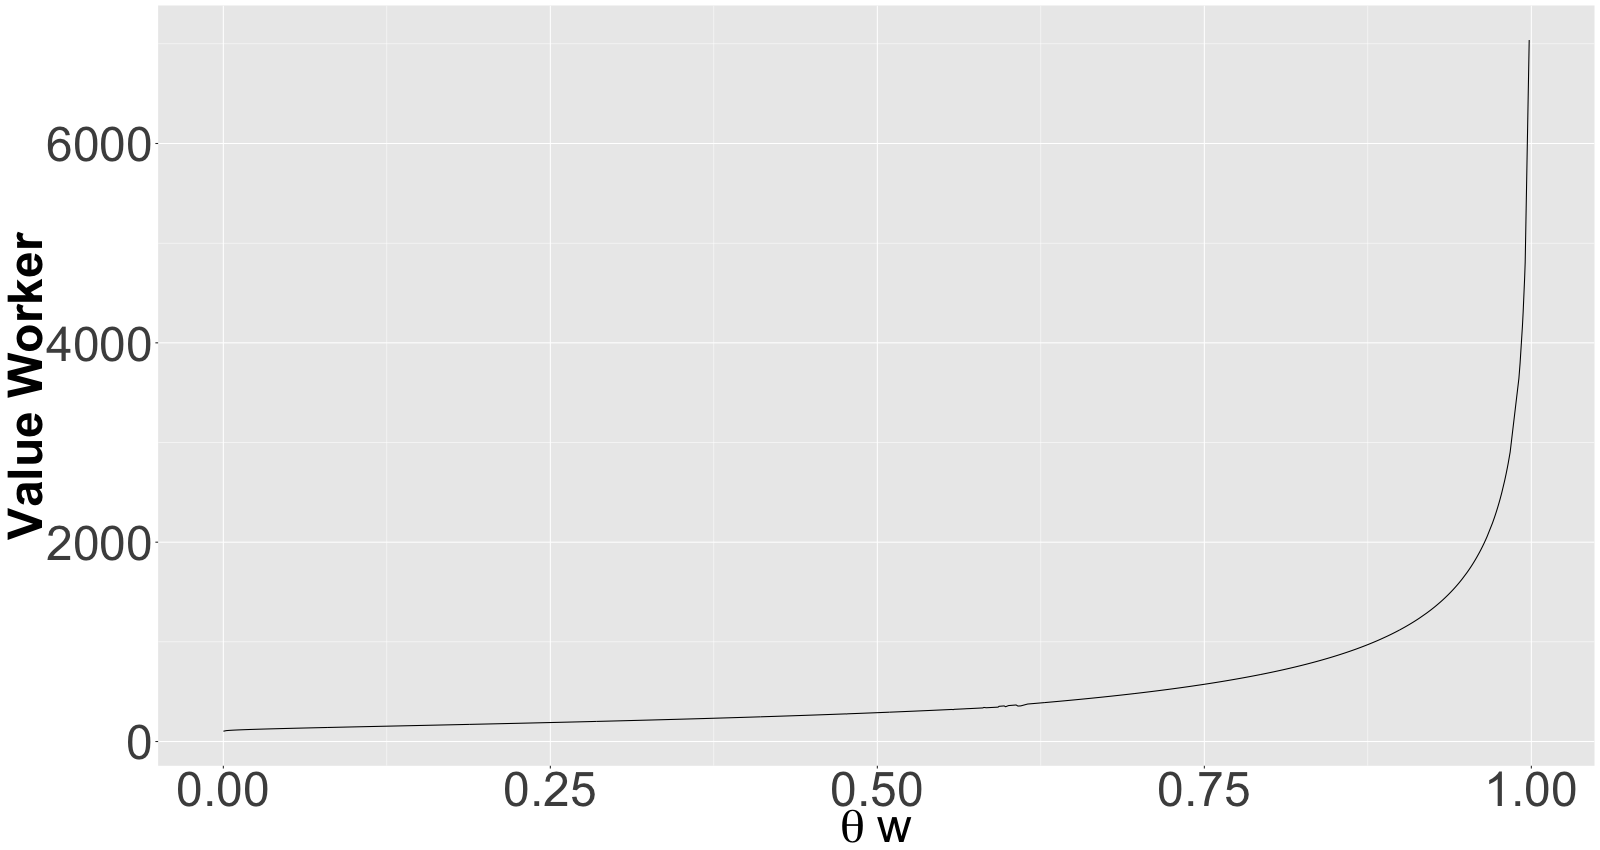
\includegraphics[width=1\textwidth]{/Users/rodrigoazuero/Dropbox/OptmalTaxationShared/Data/git/OptimalTaxation/TheoreticalMoments/ValueWorkerPercentiles.png}

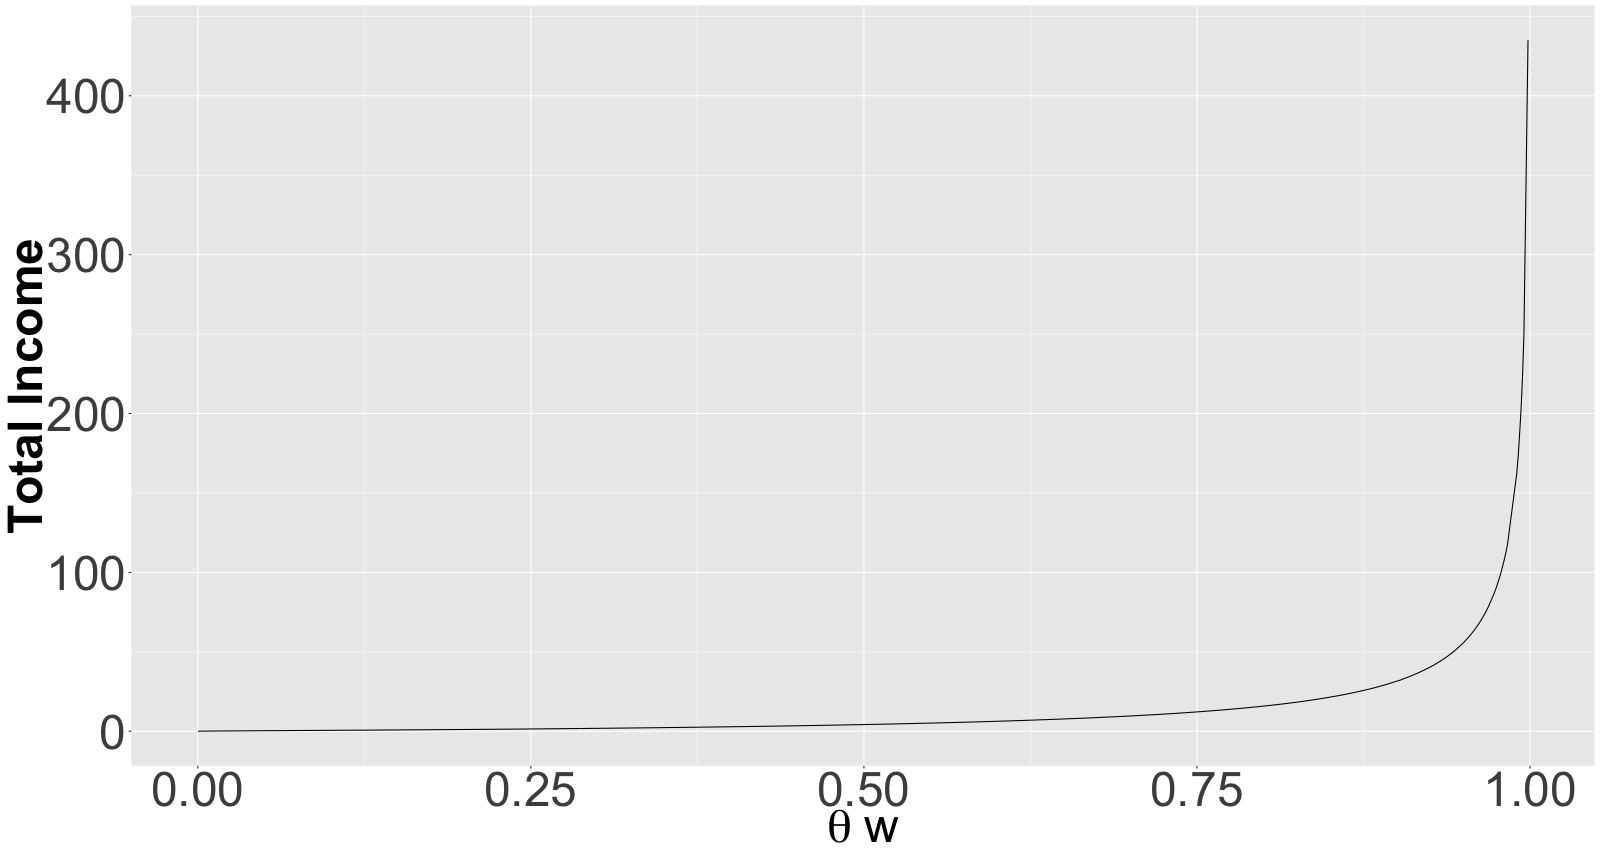
\includegraphics[width=1\textwidth]{/Users/rodrigoazuero/Dropbox/OptmalTaxationShared/Data/git/OptimalTaxation/TheoreticalMoments/TotalIncomePercentiles.png}



\end{document}


